
\documentclass[notes,11pt, aspectratio=169]{beamer}

\usepackage{pgfpages}
\usepackage{mdwlist}
% These slides also contain speaker notes. You can print just the slides,
% just the notes, or both, depending on the setting below. Comment out the want
% you want.
\setbeameroption{hide notes} % Only slide
%\setbeameroption{show only notes} % Only notes
%\setbeameroption{show notes on second screen=right} % Both

\usepackage{helvet}
\usepackage[default]{lato}
\usepackage{array}
\usepackage{tgbonum}
\usepackage[sfdefault]{FiraSans} %% option 'sfdefault' activates Fira Sans as the default text font
\usepackage[T1]{fontenc}
\renewcommand*\oldstylenums[1]{{\firaoldstyle #1}}

\usepackage{tikz}
\usepackage{verbatim}
\setbeamertemplate{note page}{\pagecolor{yellow!5}\insertnote}
\usetikzlibrary{positioning}
\usetikzlibrary{snakes}
\usetikzlibrary{calc}
\usetikzlibrary{arrows}
\usetikzlibrary{decorations.markings}
\usetikzlibrary{shapes.misc}
\usetikzlibrary{matrix,shapes,arrows,fit,tikzmark}
\usepackage{amsmath}
\usepackage{mathpazo}
\usepackage{hyperref}
\usepackage{lipsum}
\usepackage{multimedia}
\usepackage{graphicx}
\usepackage{multirow}
\usepackage{graphicx}
\usepackage{dcolumn}
\usepackage{bbm}
\newcolumntype{d}[0]{D{.}{.}{5}}

\usepackage{changepage}
\usepackage{appendixnumberbeamer}
\newcommand{\beginbackup}{
   \newcounter{framenumbervorappendix}
   \setcounter{framenumbervorappendix}{\value{framenumber}}
   \setbeamertemplate{footline}
   {
     \leavevmode%
     \hline
     box{%
       \begin{beamercolorbox}[wd=\paperwidth,ht=2.25ex,dp=1ex,right]{footlinecolor}%
%         \insertframenumber  \hspace*{2ex} 
       \end{beamercolorbox}}%
     \vskip0pt%
   }
 }
\newcommand{\backupend}{
   \addtocounter{framenumbervorappendix}{-\value{framenumber}}
   \addtocounter{framenumber}{\value{framenumbervorappendix}} 
}


\usepackage{graphicx}
\usepackage[space]{grffile}
\usepackage{booktabs}
\newcommand\independent{\protect\mathpalette{\protect\independenT}{\perp}}
\def\independenT#1#2{\mathrel{\rlap{$#1#2$}\mkern2mu{#1#2}}}
\DeclareMathOperator{\Supp}{Supp}

% These are my colors -- there are many like them, but these ones are mine.
\definecolor{blue}{RGB}{0,114,178}
\definecolor{red}{RGB}{213,94,0}
\definecolor{yellow}{RGB}{240,228,66}
\definecolor{green}{RGB}{0,158,115}

\hypersetup{
  colorlinks=false,
  linkbordercolor = {white},
  linkcolor = {blue}
}


%% I use a beige off white for my background
\definecolor{MyBackground}{RGB}{255,253,218}

%% Uncomment this if you want to change the background color to something else
%\setbeamercolor{background canvas}{bg=MyBackground}

%% Change the bg color to adjust your transition slide background color!
\newenvironment{transitionframe}{
  \setbeamercolor{background canvas}{bg=yellow}
  \begin{frame}}{
    \end{frame}
}

\setbeamercolor{frametitle}{fg=blue}
\setbeamercolor{title}{fg=black}
\setbeamertemplate{footline}[frame number]
\setbeamertemplate{navigation symbols}{} 
\setbeamertemplate{itemize items}{-}
\setbeamercolor{itemize item}{fg=blue}
\setbeamercolor{itemize subitem}{fg=blue}
\setbeamercolor{enumerate item}{fg=blue}
\setbeamercolor{enumerate subitem}{fg=blue}
\setbeamercolor{button}{bg=MyBackground,fg=blue,}



% If you like road maps, rather than having clutter at the top, have a roadmap show up at the end of each section 
% (and after your introduction)
% Uncomment this is if you want the roadmap!
% \AtBeginSection[]
% {
%    \begin{frame}
%        \frametitle{Roadmap of Talk}
%        \tableofcontents[currentsection]
%    \end{frame}
% }
\setbeamercolor{section in toc}{fg=blue}
\setbeamercolor{subsection in toc}{fg=red}
\setbeamersize{text margin left=1em,text margin right=1em} 

\newenvironment{wideitemize}{\itemize\addtolength{\itemsep}{10pt}}{\enditemize}

\usepackage{environ}
\NewEnviron{videoframe}[1]{
  \begin{frame}
    \vspace{-8pt}
    \begin{columns}[onlytextwidth, T] % align columns
      \begin{column}{.70\textwidth}
        \begin{minipage}[t][\textheight][t]
          {\dimexpr\textwidth}
          \vspace{8pt}
          \hspace{4pt} {\Large \sc \textcolor{blue}{#1}}
          \vspace{8pt}
          
          \BODY
        \end{minipage}
      \end{column}%
      \hfill%
      \begin{column}{.38\textwidth}
        \colorbox{green!20}{\begin{minipage}[t][1.2\textheight][t]
            {\dimexpr\textwidth}
            Face goes here
          \end{minipage}}
      \end{column}%
    \end{columns}
  \end{frame}
}

\title[]{\textcolor{blue}{Duration Models}}
\author[PGP]{}
\institute[FRBNY]{\small{Paul Goldsmith-Pinkham}}
\date{\today}


\begin{document}

%%% TIKZ STUFF
\tikzset{   
        every picture/.style={remember picture,baseline},
        every node/.style={anchor=base,align=center,outer sep=1.5pt},
        every path/.style={thick},
        }
\newcommand\marktopleft[1]{%
    \tikz[overlay,remember picture] 
        \node (marker-#1-a) at (-.3em,.3em) {};%
}
\newcommand\markbottomright[2]{%
    \tikz[overlay,remember picture] 
        \node (marker-#1-b) at (0em,0em) {};%
}
\tikzstyle{every picture}+=[remember picture] 
\tikzstyle{mybox} =[draw=black, very thick, rectangle, inner sep=10pt, inner ysep=20pt]
\tikzstyle{fancytitle} =[draw=black,fill=red, text=white]
%%%% END TIKZ STUFF

% Title Slide
\begin{frame}
\maketitle

\end{frame}


\begin{frame}{Today's topic: duration models}
  \begin{columns}[T] % align columns
    \begin{column}{.7\textwidth}
      \begin{wideitemize}
      \item First question is: what's a duration model?
      \item Second question: why do we care?
      \item Third question: what are ways to estimate them? What are
        estimands that are identified in these settings?
      \end{wideitemize}
    \end{column}%
  \hfill%
  \begin{column}{.4\textwidth}
  \end{column}
\end{columns}
\end{frame}

\begin{frame}{What's a duration model?}
  \begin{wideitemize}
  \item A duration model is just what is sounds like -- a model
    relating to duration of an event
  \item Why would we need a special model for this?
    \begin{enumerate}
    \item Data measurement: measuring durations accurately is challenging!
    \item Estimation: the mapping between theory and estimation can
      require more sophisticated models
    \end{enumerate}
  \item We'll start by just discussing what's special about durations
  \end{wideitemize}
\end{frame}


\begin{frame}{First, some examples}
  \begin{wideitemize}
  \item Lancaster (1979) - unemployment spells
    \begin{itemize}
    \item $t=0$: unemployment begins
    \item Spell ends: employment
    \end{itemize}
  \item Galiani, Gertler and Schargrodsky (2005) - privatizing water service 
    \begin{itemize}
    \item $t=0$: the year 1990
    \item Spell ends: water service privatized      
    \end{itemize}
  \item Palmer (2015) - mortgage default
    \begin{itemize}
    \item $t = 0$: Mortgage origination
    \item Spell ends: mortgage default
    \end{itemize}
  \item Rose (2020) - supervised release
    \begin{itemize}
    \item $t = 0$: Release 
    \item Spell ends:  New arrest or revocation
    \end{itemize}
  \end{wideitemize}
\end{frame}


\begin{frame}{More examples}
  \begin{wideitemize}
  \item Engle and Russell (1998) -- Irregularly spaced transaction data
    \begin{itemize}
    \item $\{t_{0}, t_{1}, \ldots, t_{n}, \ldots \}$ denote arrival times of transactions
    \item Condition on previous events -- ``autoregressive conditional duration'' models
    \end{itemize}
  \item Carlson et al. (2015) - bankruptcy
    \begin{itemize}
    \item $t = 0$ retirement from NFL
    \item Spell ends: bankruptcy filing
    \end{itemize}
  \item Goldsmith-Pinkham \& Gilbukh (2021) - moving houses
    \begin{itemize}
    \item $t = 0$ buy a home
    \item Spell ends: buy a new home
    \end{itemize}
  \end{wideitemize}
\end{frame}



\begin{frame}{Running example}
  \begin{wideitemize}
  \item One very common duration is the duration of tenure in housing
  \item Let $Y_{i}$ denote the length of time that individual $i$ lives in their home.
    \begin{itemize}
    \item If we have better data, we can even consider $Y_{is}$ to be the length of time that individual $i$ lives in their home in spell $s$
    \item Multiple spells, e.g. panel data
    \end{itemize}
  \item A number of notable things could affect this tenure:
    \begin{itemize}
    \item Age of the individuals
    \item The housing cycle
    \item The business cycle
    \item Whether or not they are homeowners
    \end{itemize}
  \end{wideitemize}
\end{frame}

\begin{frame}{Types of Duration Data we observe}
  \begin{wideitemize}
  \item The ``truth'': A single duration observed for person $i$, $Y_{i} \in [0, T]$
    \begin{itemize}
    \item In theory, the duration could be unbounded $T = \infty$, but
      could be maximally bounded (e.g. max lifetime of human)
    \end{itemize}
  \item What kind of data do we observe?
    \begin{itemize}
    \item First example is best case but given unbounded nature of $T$, unrealistic for everything
    \item For a given observation, we see spell start and spell end
    \end{itemize}
  \end{wideitemize}
  \begin{center}
    \begin{tabular}{lcc}
      Case & Start & End\\
      \midrule
      Full & $t_{0}$ & $t_{1}$\\
    \end{tabular}
    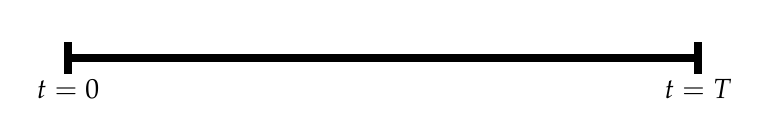
\begin{tikzpicture}[snake=zigzag, line before snake = 5mm, line after snake = 5mm, line width=1mm]
    % draw horizontal line   
    \draw (0,0) -- (8,0);
    %\draw[->] (8,0) -- (9,0);

    % \draw (0,.95) -- (1,.95);
    % \draw[snake] (1,.95) -- (3,.95);
    % \draw (3,.95) -- (4,.95);
    % \draw[red] (4,.95) -- (8,.95);
    % \draw[->] (8,.95) -- (9,.95);

    % draw vertical lines
    \foreach \x in {8}
      \draw (\x cm,.205) -- (\x cm,-.205);
    % \foreach \x in {4}
    %   \draw (\x cm,{.95+(.205)}) -- (\x cm,{.95-(.205)});
    % \foreach \x in {0}
    % \draw (\x cm,{.95+(.205)}) -- (\x cm,{0-(.205)});
    \foreach \x in {0}      
      \draw (\x cm,{0+(.205)}) -- (\x cm,{0-(.205)});
      
    % draw nodes
      \draw (0,0) node[below=.105] {}  node[below=.105] {$t=0$};
      \draw (8,0) node[below=.105] {}  node[below=.105] {$t=T$};      
      \draw (0,0) node[below=.105] {}  node[left=.105] {};      
    % \draw (0,0.95) node[below=.105] {} node[above=.105] {} node[left=.105] {\textcolor{red}{Treatment}};
    % \draw (4,.95) node[below=.105] {} node[above=.105] {} node[below=.105] {Policy Treatment};
    \draw (8,0) node[below=.105] {} node[above=.105] {} node[below=.105] {};
  \end{tikzpicture}
\end{center}
\end{frame}


\begin{frame}{Types of Duration Data we observe}
  \begin{wideitemize}
  \item Sometimes we can't see everything -- sampling costs, or
    limitations on time
    \begin{itemize}
    \item You may write your paper before people decide to move!
    \end{itemize}
  \item This can create a form of right-censoring
    \begin{itemize}
    \item For a given observation, we see spell start and spell end
      for most individuals (observed before $c$, or $c_{i}$)
    \item For those who have not had their spell end by $c$ or
      $c_{i}$, we only observe the censoring period
    \end{itemize}
  \item \emph{If this censoring can be viewed as random}, this is
    (parametrically) addressable
  \end{wideitemize}
  \begin{center}
    \begin{tabular}{lcc}
      Case & Start & End\\
      \midrule
      Full & $t_{0}$ & $t_{1}$\\
      Right-Censor & $t_{0}$ & $\min\{{t_{1}, c}\}$\\      
    \end{tabular}
    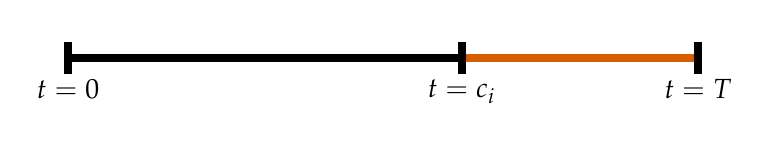
\begin{tikzpicture}[snake=zigzag, line before snake = 5mm, line after snake = 5mm, line width=1mm]
    % draw horizontal line   
      \draw (0,0) -- (5,0);
    \draw[red] (5,0) -- (8,0);      
    %\draw[->] (8,0) -- (9,0);

    % \draw (0,.95) -- (1,.95);
    % \draw[snake] (1,.95) -- (3,.95);
    % \draw (3,.95) -- (4,.95);
    % \draw[red] (4,.95) -- (8,.95);
    % \draw[->] (8,.95) -- (9,.95);

    % draw vertical lines
    \foreach \x in {8}
      \draw (\x cm,.205) -- (\x cm,-.205);
     \foreach \x in {5}
       \draw (\x cm,{0+(.205)}) -- (\x cm,{0-(.205)});
    % \foreach \x in {0}
    % \draw (\x cm,{.95+(.205)}) -- (\x cm,{0-(.205)});
    \foreach \x in {0}      
      \draw (\x cm,{0+(.205)}) -- (\x cm,{0-(.205)});
      
    % draw nodes
      \draw (0,0) node[below=.105] {}  node[below=.105] {$t=0$};
      \draw (8,0) node[below=.105] {}  node[below=.105] {$t=T$};
      \draw (5,0) node[below=.105] {}  node[below=.105] {$t=c_{i}$};            
      \draw (0,0) node[below=.105] {}  node[left=.105] {};      
    % \draw (0,0.95) node[below=.105] {} node[above=.105] {} node[left=.105] {\textcolor{red}{Treatment}};
    % \draw (4,.95) node[below=.105] {} node[above=.105] {} node[below=.105] {Policy Treatment};
    \draw (8,0) node[below=.105] {} node[above=.105] {} node[below=.105] {};
  \end{tikzpicture}
\end{center}
\end{frame}



\begin{frame}{Types of Duration Data we observe}
  \begin{wideitemize}
  \item Sometimes it's even less information in our sampling scheme
  \item We know when the spells began, but can only identify whether
    or not exits occured as of period $c_{i}$
    \begin{itemize}
    \item Easy to envision data sampling like this -- checking in on a
      pool of individuals, and identifying whether they stuck around
    \end{itemize}
  \item This leaves us with less information, but so
    long as the censoring (e.g. the time of check-in) is sufficiently
    random, also addressable
  \end{wideitemize}
  \begin{center}
    \begin{tabular}{lcc}
      Case & Start & End\\
      \midrule
      Full & $t_{0}$ & $t_{1}$\\
      Right-Censor & $t_{0}$ & $\min\{{t_{1}, c_{i}}\}$\\
      Indicator   & $t_{0}$ & $1(Y_{i} < c)$\\            
    \end{tabular}
    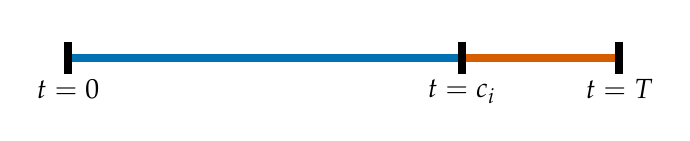
\begin{tikzpicture}[snake=zigzag, line before snake = 5mm, line after snake = 5mm, line width=1mm]
    % draw horizontal line   
      \draw[blue] (0,0) -- (5,0);
    \draw[red] (5,0) -- (7,0);      
    %\draw[->] (8,0) -- (9,0);

    % \draw (0,.95) -- (1,.95);
    % \draw[snake] (1,.95) -- (3,.95);
    % \draw (3,.95) -- (4,.95);
    % \draw[red] (4,.95) -- (8,.95);
    % \draw[->] (8,.95) -- (9,.95);

    % draw vertical lines
    \foreach \x in {7}
      \draw (\x cm,.205) -- (\x cm,-.205);
    % \foreach \x in {4}
    %   \draw (\x cm,{.95+(.205)}) -- (\x cm,{.95-(.205)});
    % \foreach \x in {0}
    % \draw (\x cm,{.95+(.205)}) -- (\x cm,{0-(.205)});
    \foreach \x in {5}      
      \draw (\x cm,{0+(.205)}) -- (\x cm,{0-(.205)});
    \foreach \x in {0}      
      \draw (\x cm,{0+(.205)}) -- (\x cm,{0-(.205)});
      
    % draw nodes
      \draw (0,0) node[below=.105] {}  node[below=.105] {$t=0$};
      \draw (7,0) node[below=.105] {}  node[below=.105] {$t=T$};
      \draw (5,0) node[below=.105] {}  node[below=.105] {$t=c_{i}$};            
      \draw (0,0) node[below=.105] {}  node[left=.105] {};      
    % \draw (0,0.95) node[below=.105] {} node[above=.105] {} node[left=.105] {\textcolor{red}{Treatment}};
    % \draw (4,.95) node[below=.105] {} node[above=.105] {} node[below=.105] {Policy Treatment};
    \draw (7,0) node[below=.105] {} node[above=.105] {} node[below=.105] {};
  \end{tikzpicture}
\end{center}
\end{frame}

\begin{frame}{Stock Sampling vs. Flow Sampling}
  \begin{wideitemize}
  \item In these cases so far, we observe when the start of the duration begins
    \begin{itemize}
    \item This is called flow sampling
    \end{itemize}
  \item An alternative sampling procedure samples from the stock of existing individuals
    \begin{itemize}
    \item E.g. Stock sampling
    \end{itemize}
  \item What issues does this create? Two scenarios:
    \begin{itemize}
    \item If we observe how long the duration lasted at time of
      sampling (e.g. the start time), we still need to account for the
      sample selection from stock sampling
    \item If we don't observe the start time, creates a version of
      left-censoring
    \end{itemize}
    \vspace{-5pt}
  \item \textbf{Left-censoring creates serious problems} -- need to make
    stronger assumptions
  \end{wideitemize}
  \begin{center}
    \footnotesize
    \begin{tabular}{lcccc}
      Sampling & Case & Start & End & Adjustment\\
      \midrule
      Flow & Full & $t_{0}$ & $t_{1}$ & No \\
      Flow & Right-Censor & $t_{0}$ & $\min\{{t_{1}, c_{i}}\}$ & Yes\\
      Flow & Indicator   & $t_{0}$ & $1(Y_{i} < c)$ & Yes\\
      Stock & Full & $t_{0}$ & $t_{1}$ & Yes \\
      Stock & Right-Censor & $t_{0}$ & $\min\{{t_{1}, c_{i}}\}$ & Yes\\
      Stock & Indicator & $t_{0}$ & $\min\{{t_{1}, c_{i}}\}$ & Yes\\      
    \end{tabular}
  \end{center}
\end{frame}



\begin{frame}{Key takeaway}
  \begin{wideitemize}
  \item Understanding the sampling structure of your data is always important
    \begin{itemize}
    \item Particularly important with duration data
    \end{itemize}
  \item However, censoring problems are not unique to duration data
    \begin{itemize}
    \item E.g., wage data can be censored/truncated due to reservation wages or survey measurement
    \item However, in duration data, right-censoring is quite common 
    \end{itemize}
  \item These are important features to consider for understanding the data generating process for your sample (and the population)
  \item However, a more important question is what are you interested in?
    \begin{itemize}
    \item E.g. what is your estimand?
    \item Effect of a treatment on average length of duration? Median duration?
    \item Consider $Y_{i} = \alpha + T_{i}\beta + \epsilon_{i}$ --
      this is well-defined when $T_{i}$ is randomly assigned, but
      censoring still causes issues
    \end{itemize}
  \end{wideitemize}
\end{frame}

\begin{frame}{Consider the example of housing}
  \begin{columns}[T] % align columns
    \begin{column}{.4\textwidth}
      \begin{wideitemize}
      \item Length of time between housing transactions
      \item Sample is drawn in 2017m8, but we see every transaction
        \begin{itemize}
        \item Implication: data is censored at 2017m8, which creates different censoring horizons depending on when the home was last bought
        \end{itemize}
      \only<1>{\item We can first examine full distribution of durations}
      \only<2>{\item If we focus on 2010+ cohorts, truncation problem is obvious, but shape is not}
      \only<3>{\item If we focus on 2005+ cohorts, it's clear there's heterogeneity   }
      \only<4>{\item Censoring issue is very apparently within a given year}
      \end{wideitemize}
    \end{column}%
  \hfill%
  \begin{column}{.6\textwidth}
    \only<1>{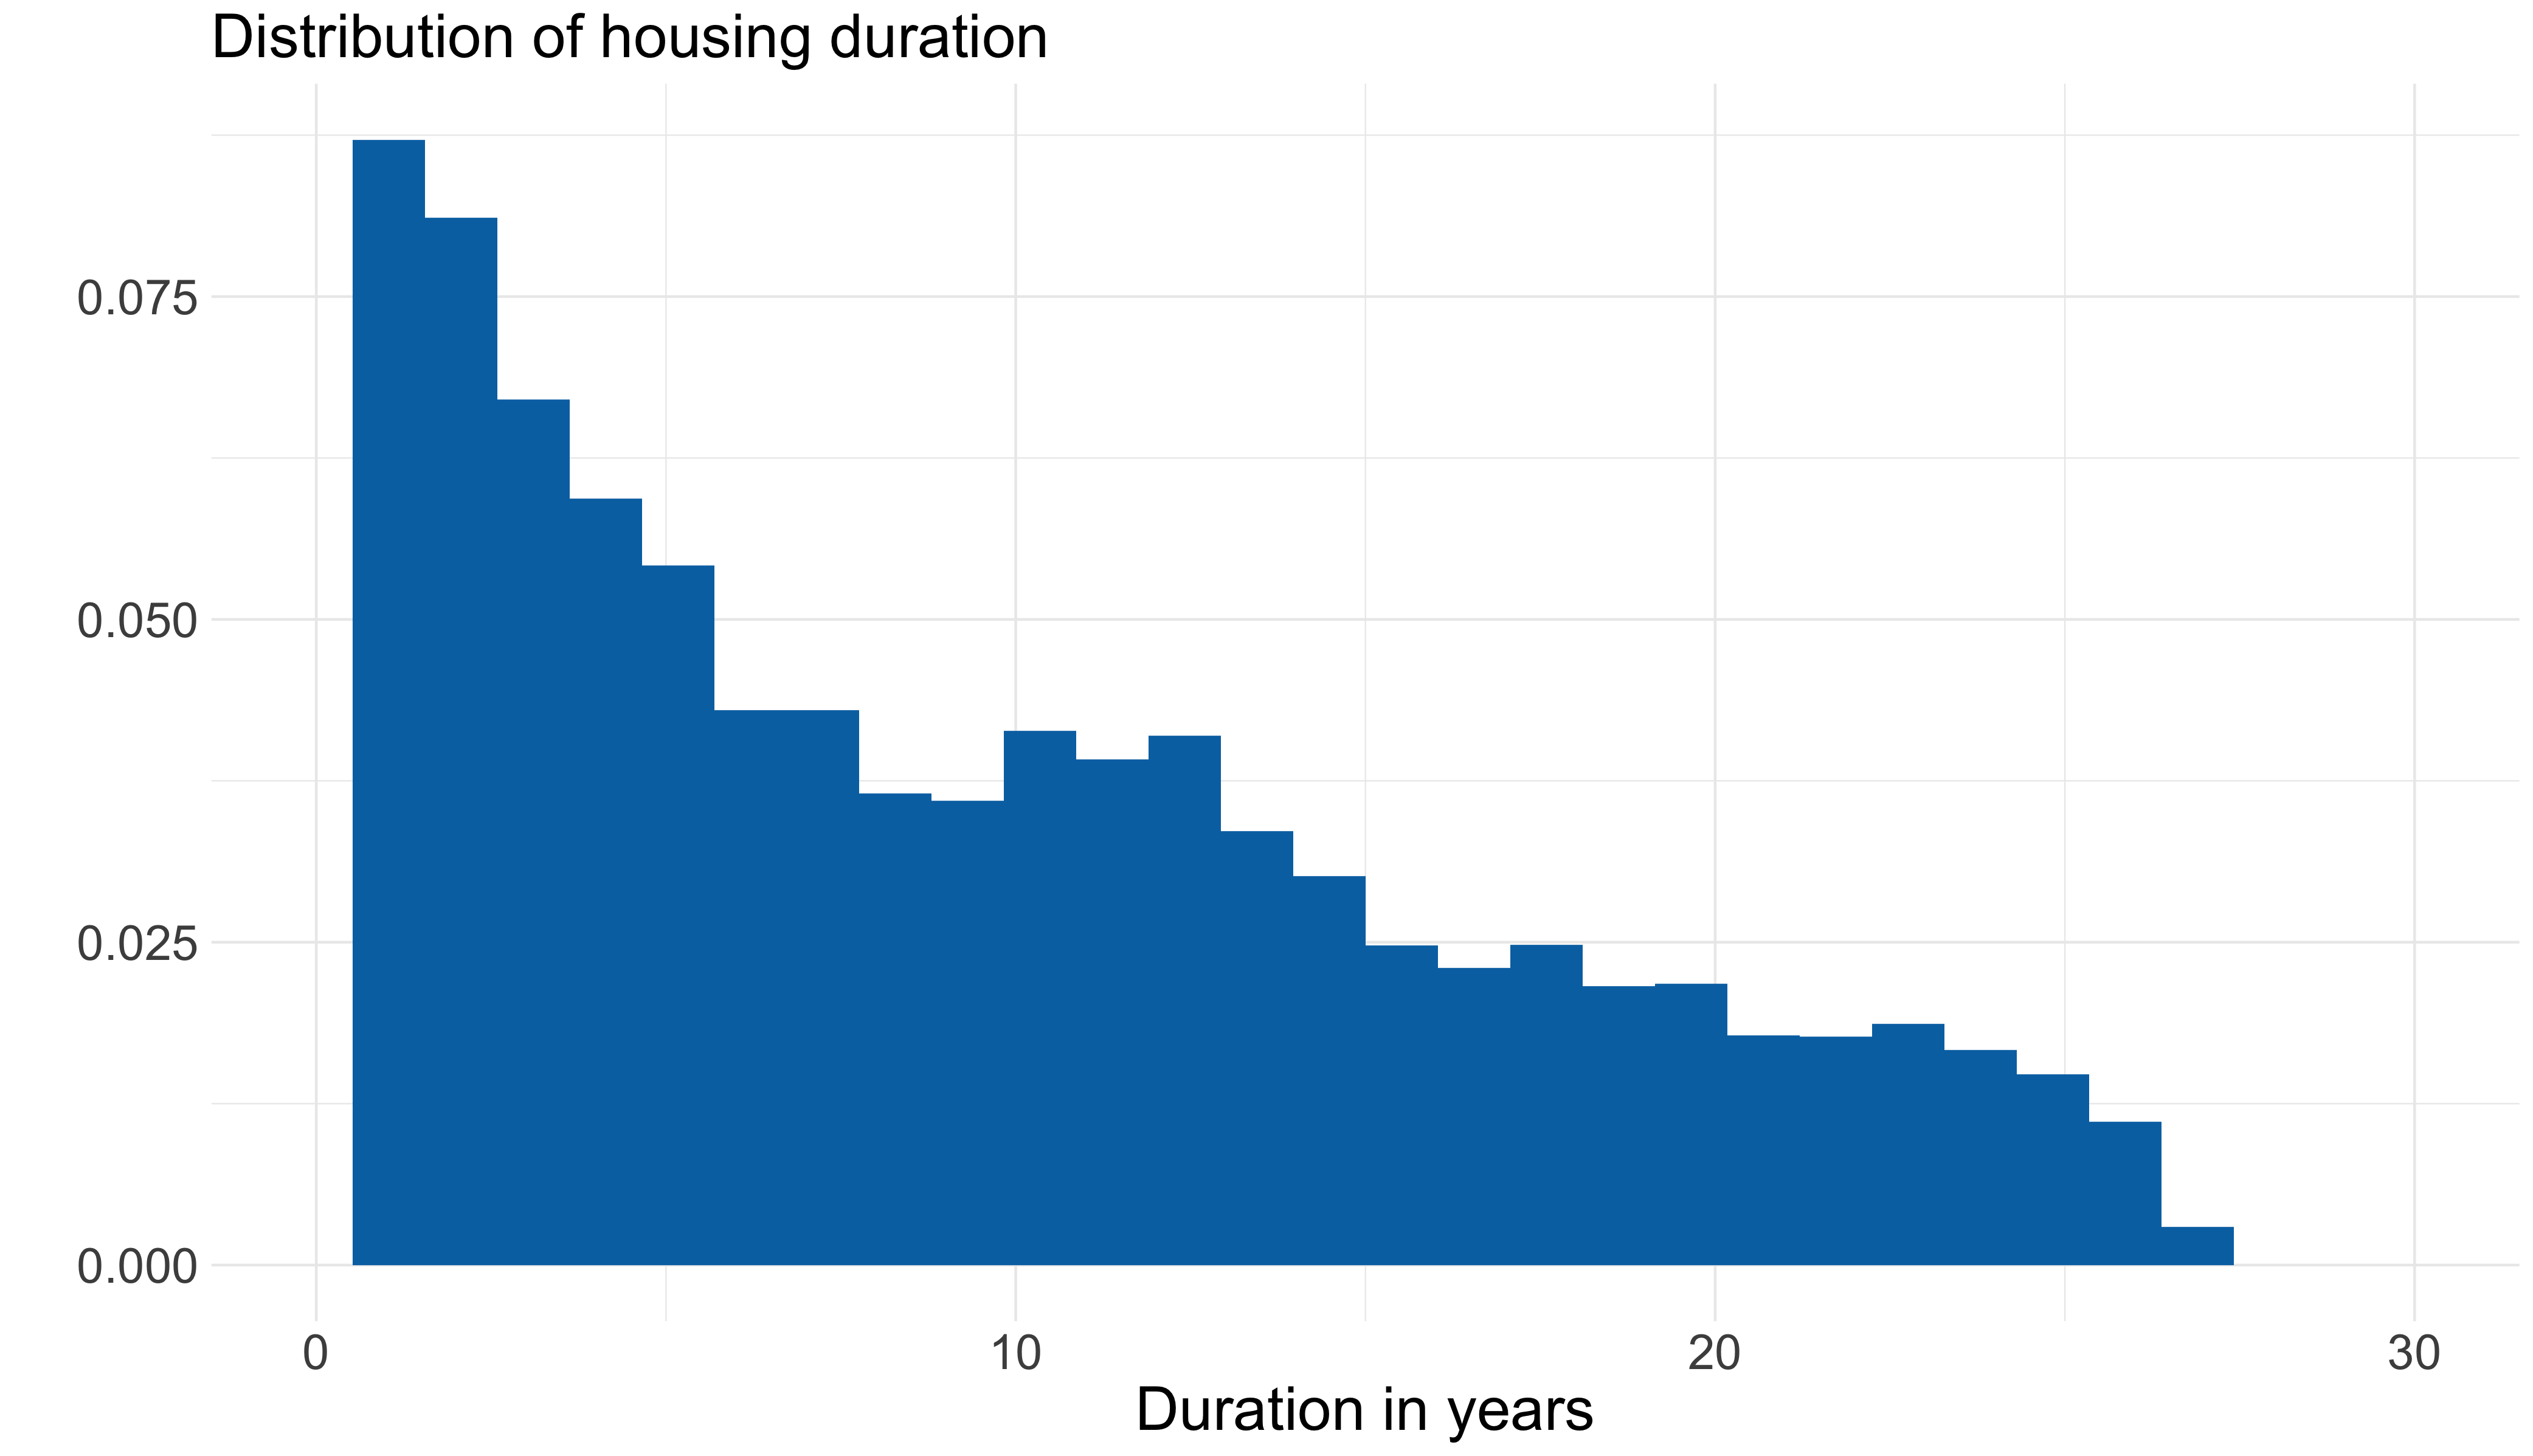
\includegraphics[width=\linewidth]{images/housing_duration_full.png}}
    \only<2>{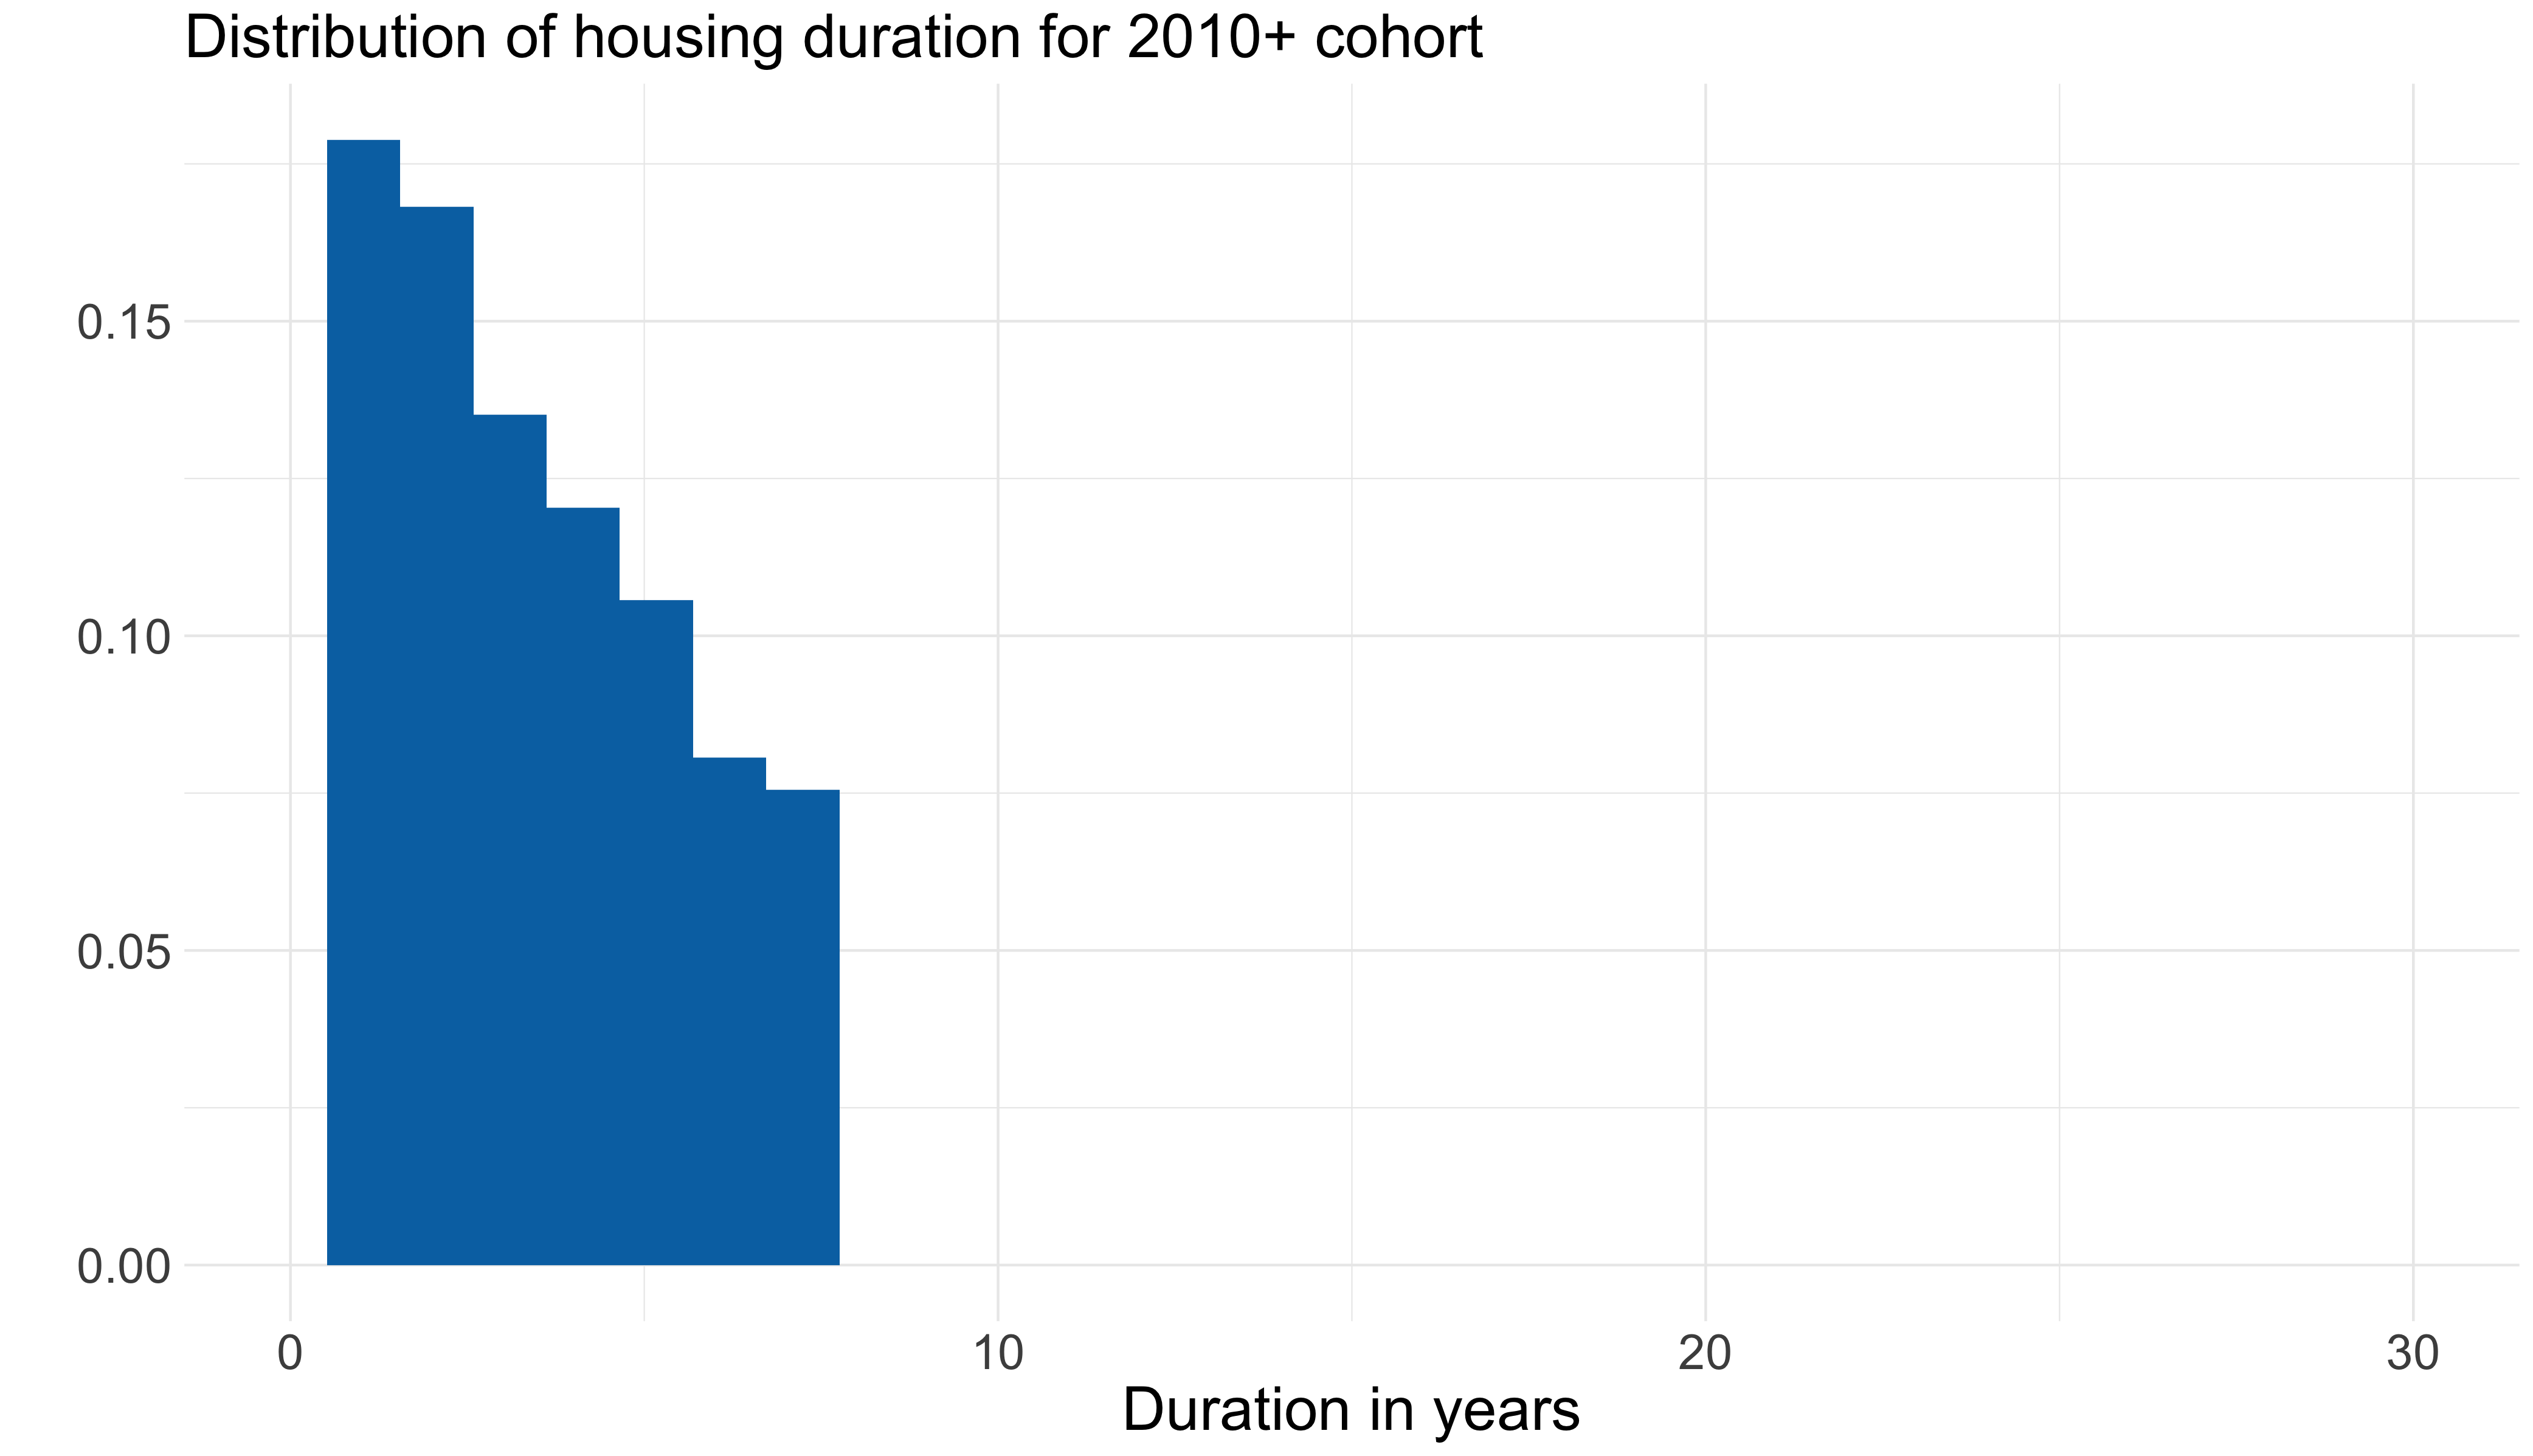
\includegraphics[width=\linewidth]{images/housing_duration_2010plus.png}}
    \only<3>{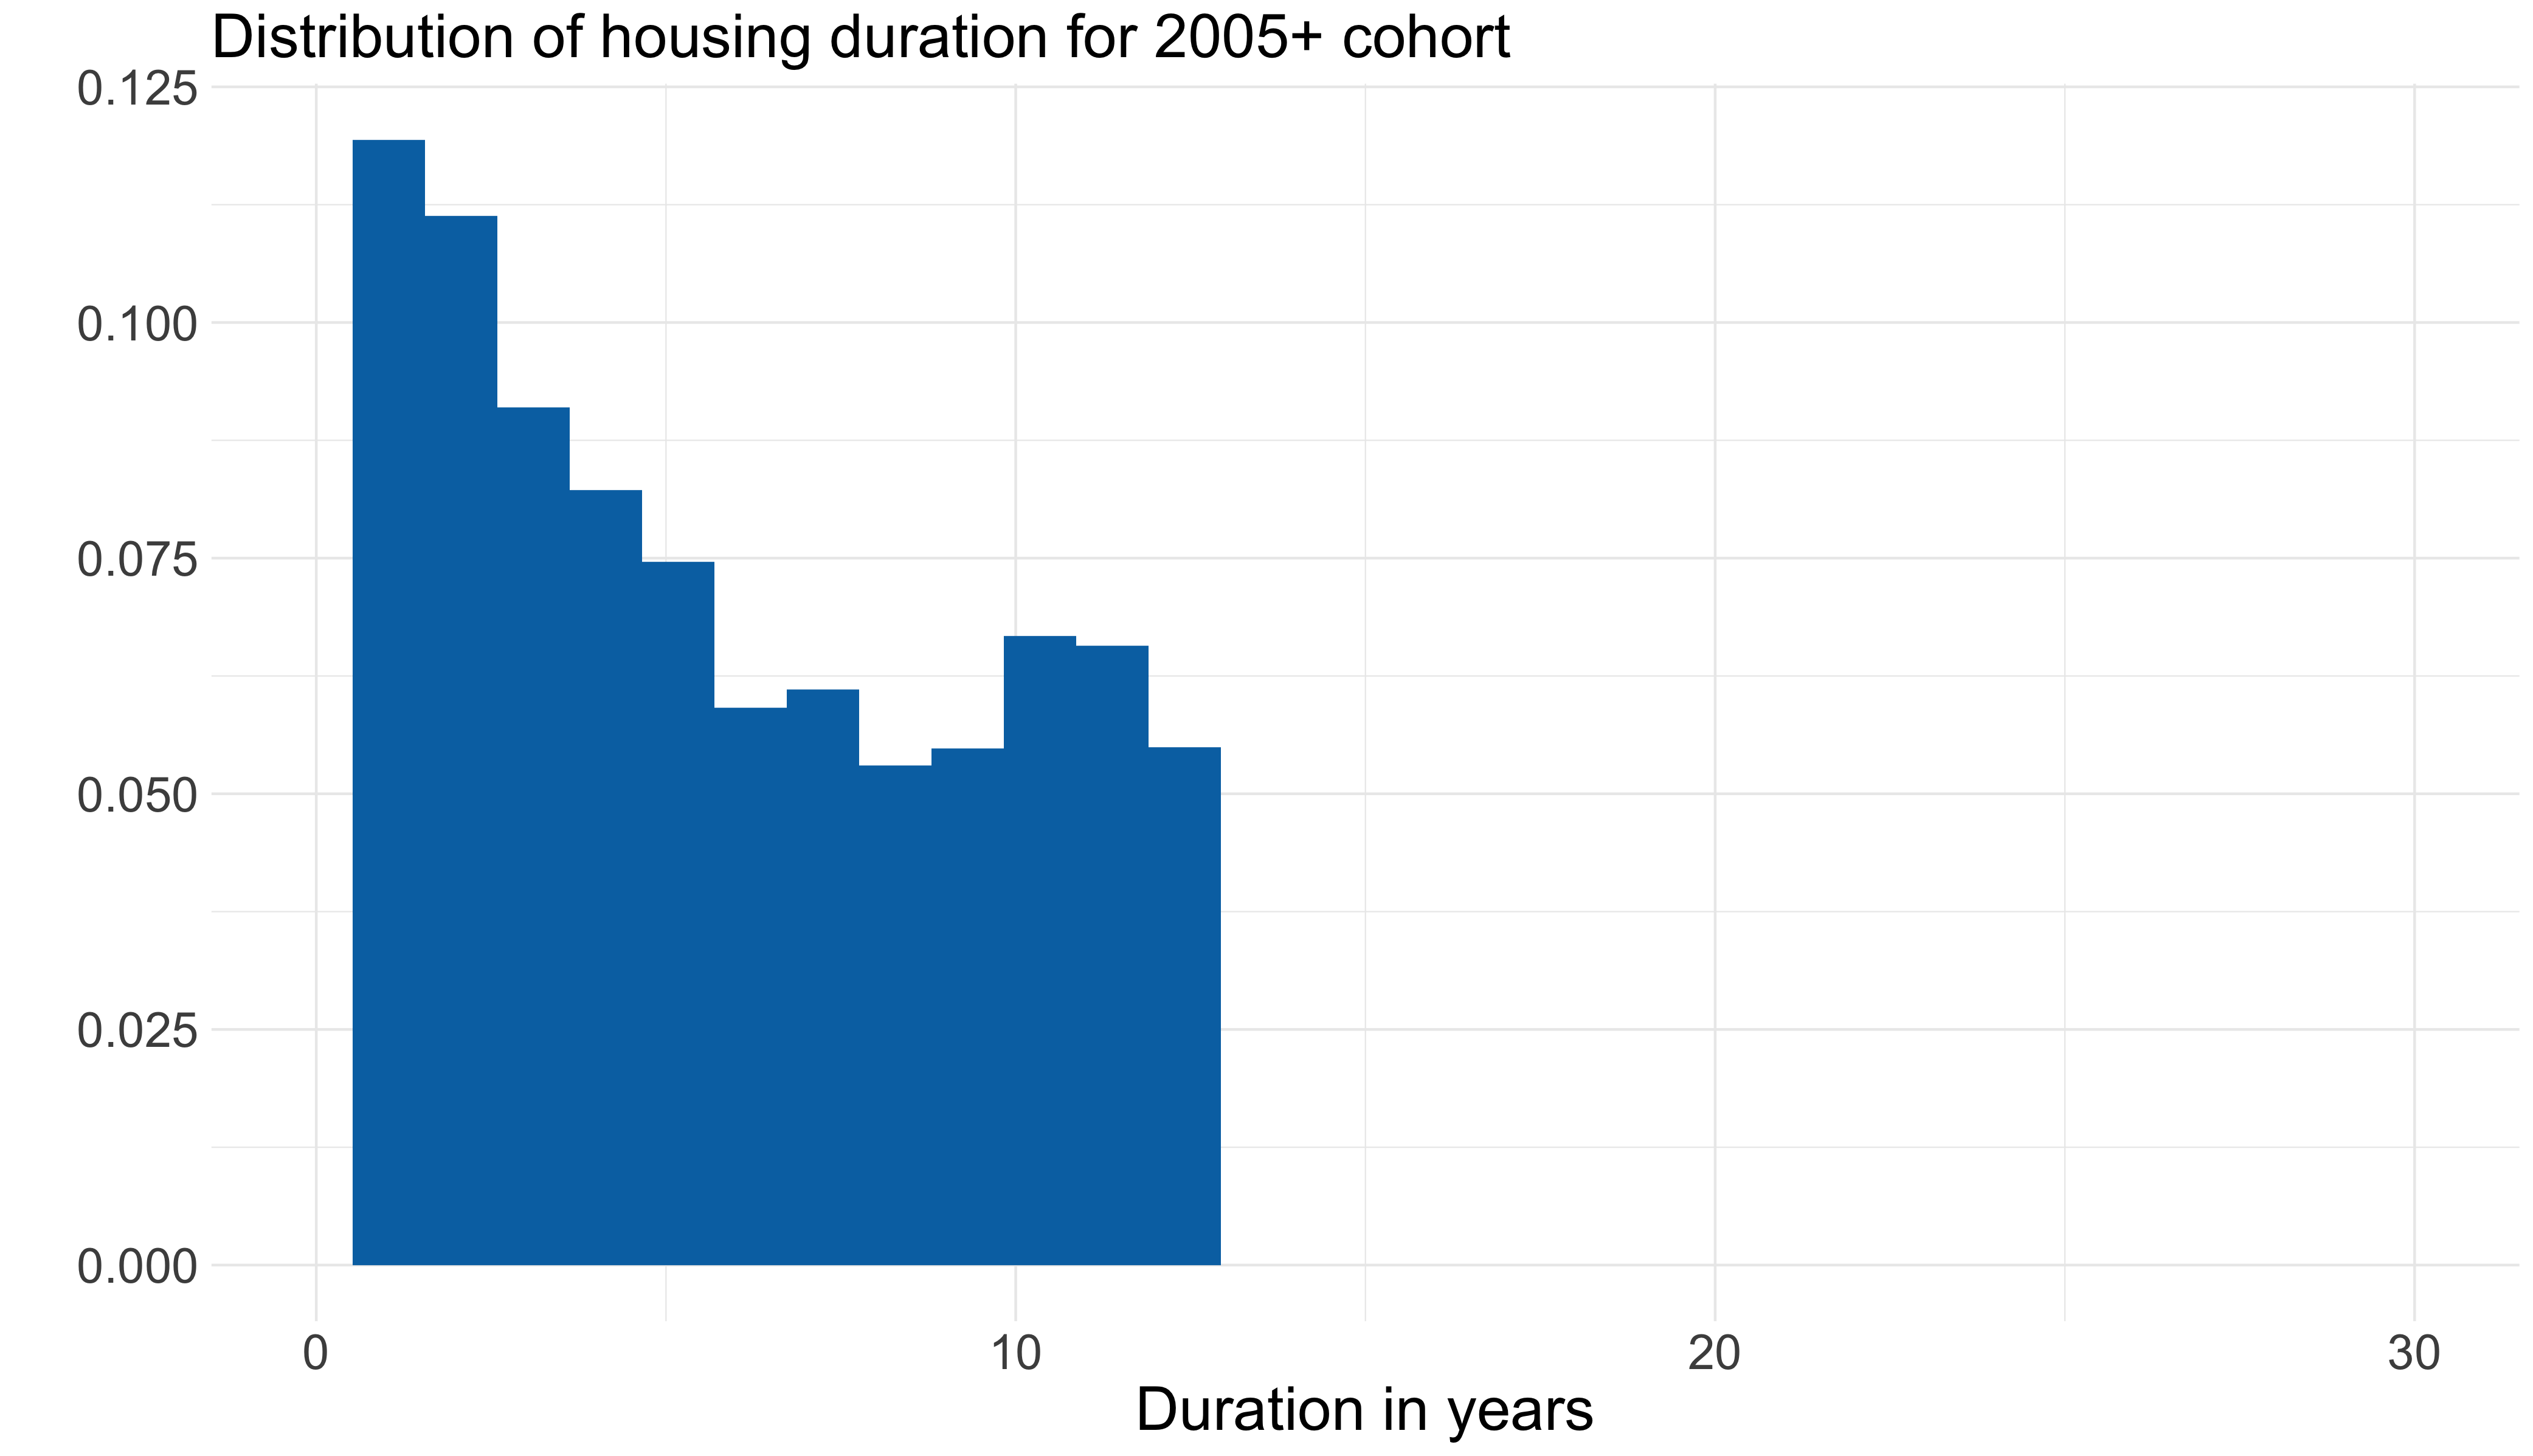
\includegraphics[width=\linewidth]{images/housing_duration_2005plus.png}}
    \only<4>{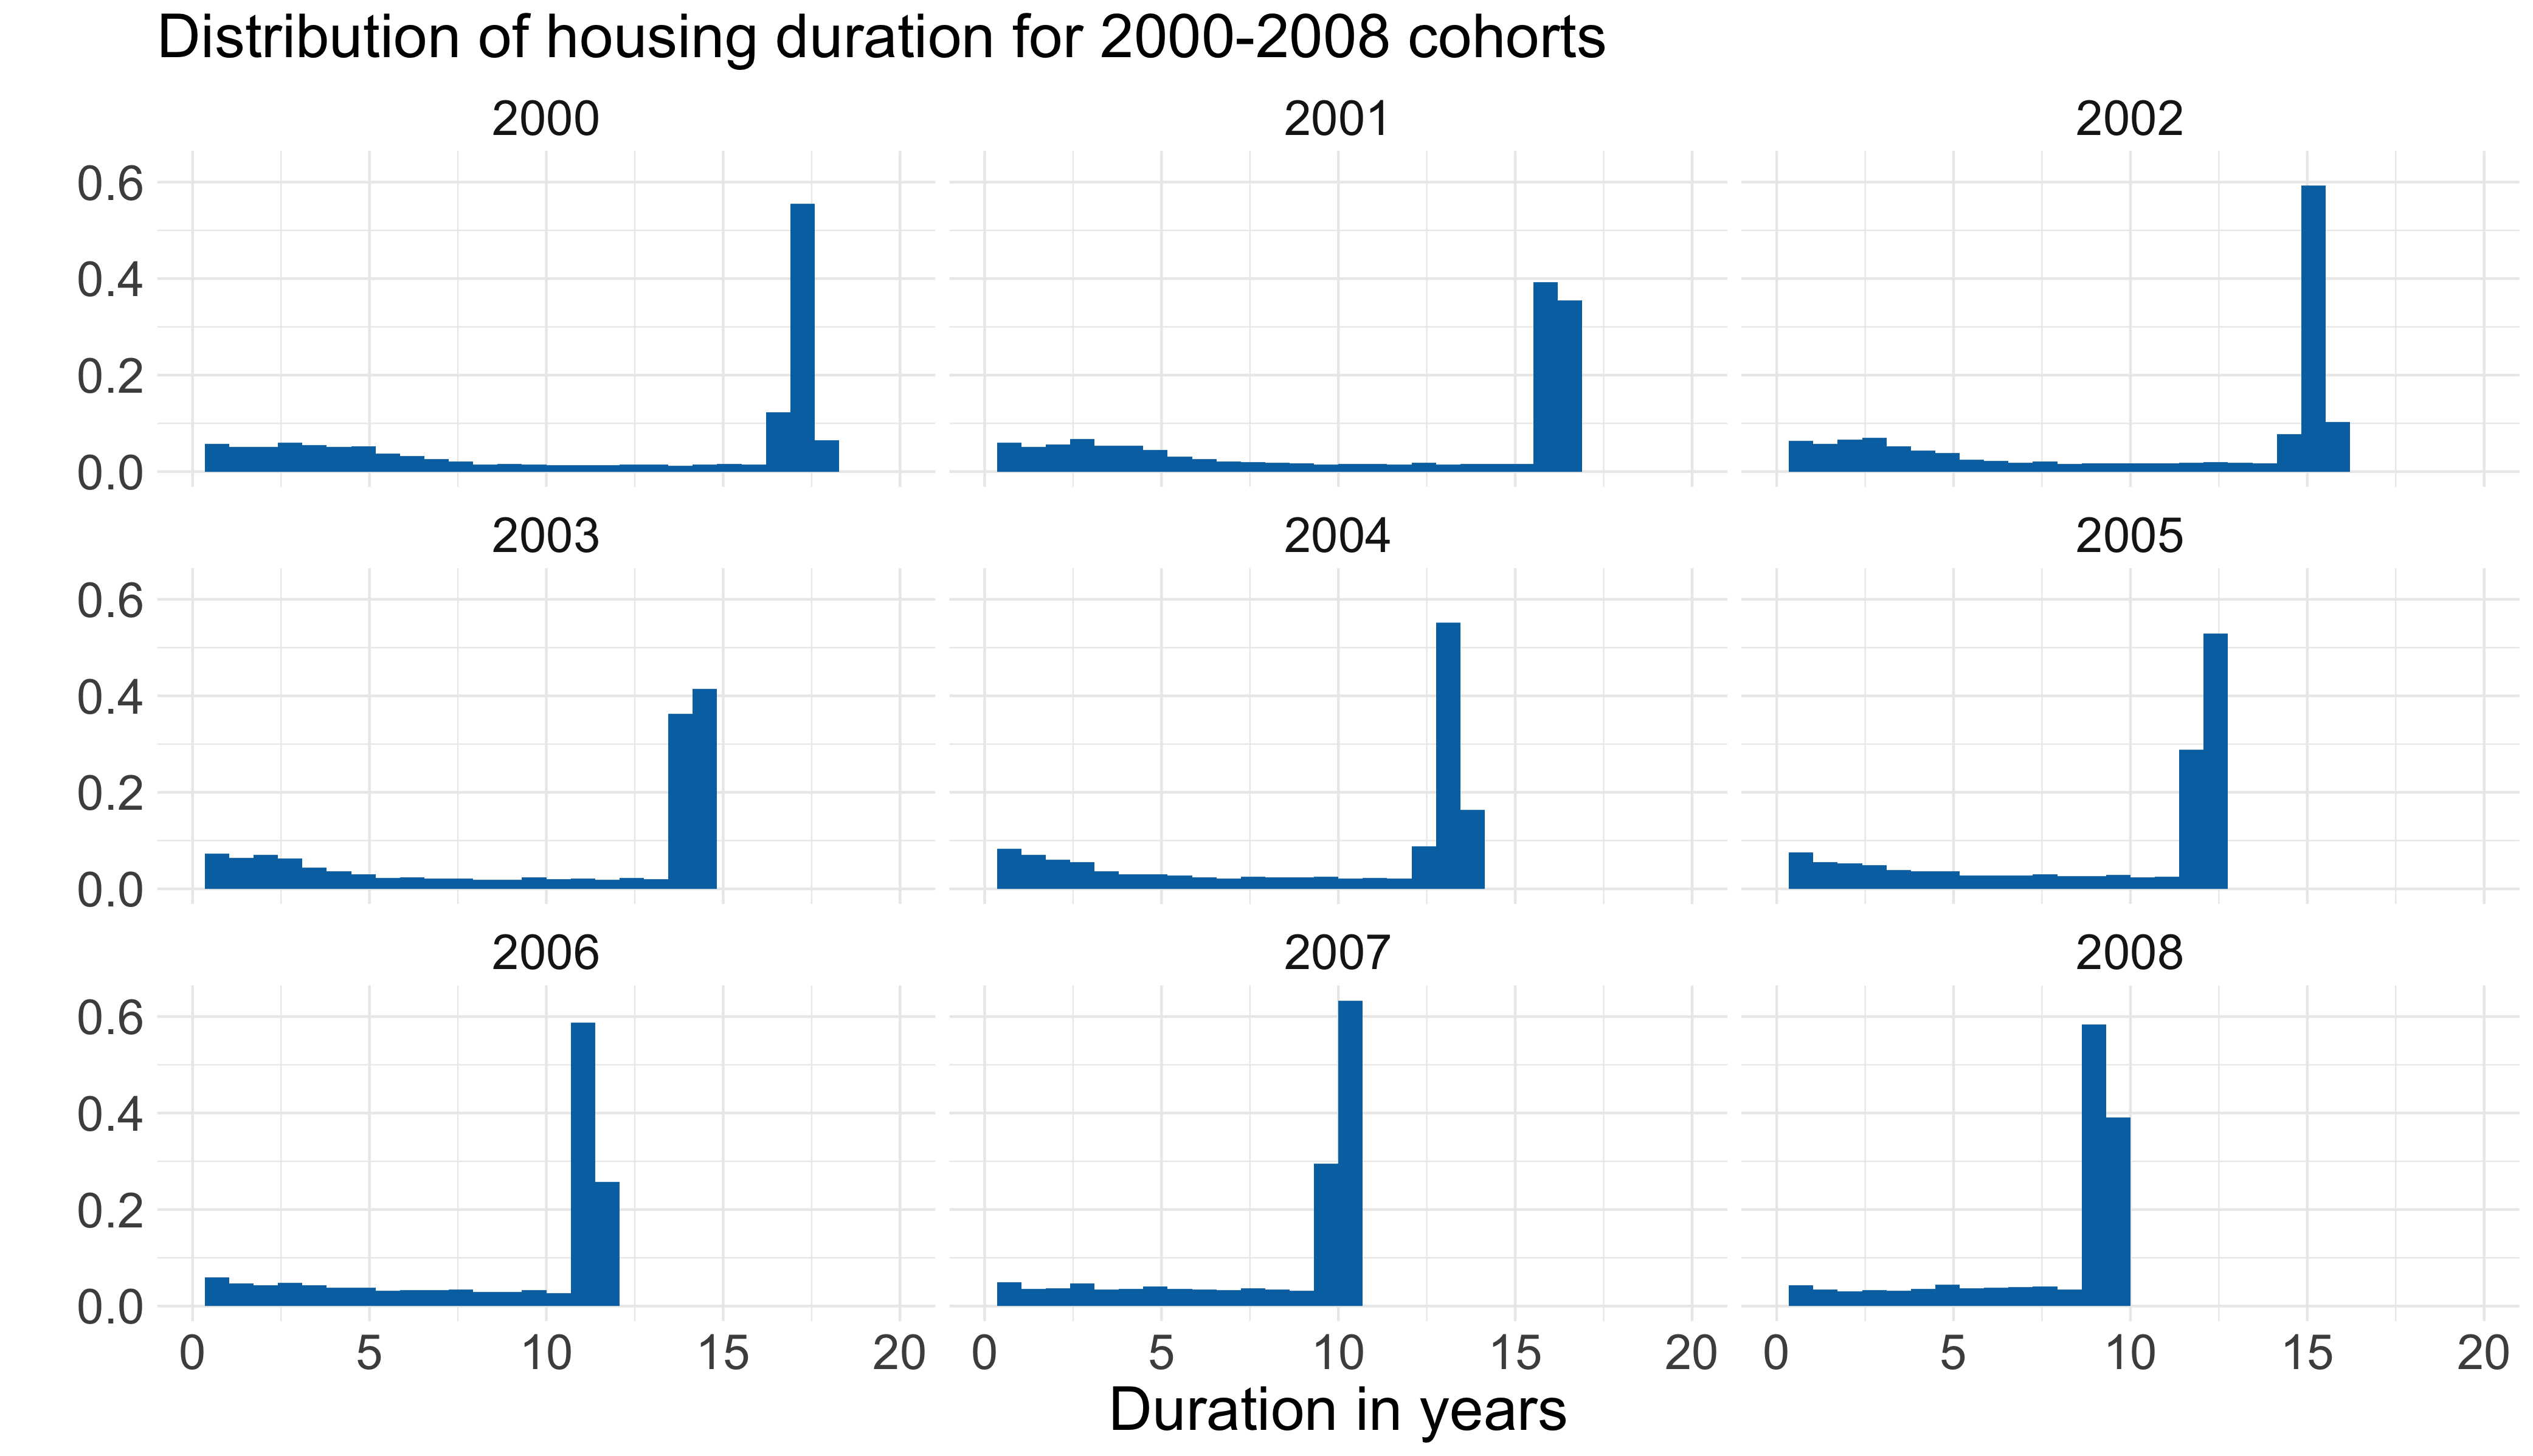
\includegraphics[width=\linewidth]{images/housing_duration_20002010_byyear.png}}    
  \end{column}
\end{columns}
\end{frame}


\begin{frame}{Consider the example of housing}
  \begin{columns}[T] % align columns
    \begin{column}{.5\textwidth}
      \begin{wideitemize}
      \item Can we calculate the average duration, without further assumptions?
        \begin{itemize}
        \item Purely non-parametrically? No. Even with random
          sampling, we don't know the DGP and the average could be
          completely unbounded
        \item Can explore this further in partial identification
        \end{itemize}
      \item If we are willing to make more assumptions (next), then yes!
      \item Before we do that -- worth recognizing that there are
        other estimands that we can identify
        \begin{itemize}
        \item E.g., the quantiles -- for 2000 cohort, the median
        \end{itemize}
      \end{wideitemize}
    \end{column}%
  \hfill%
  \begin{column}{.5\textwidth}
    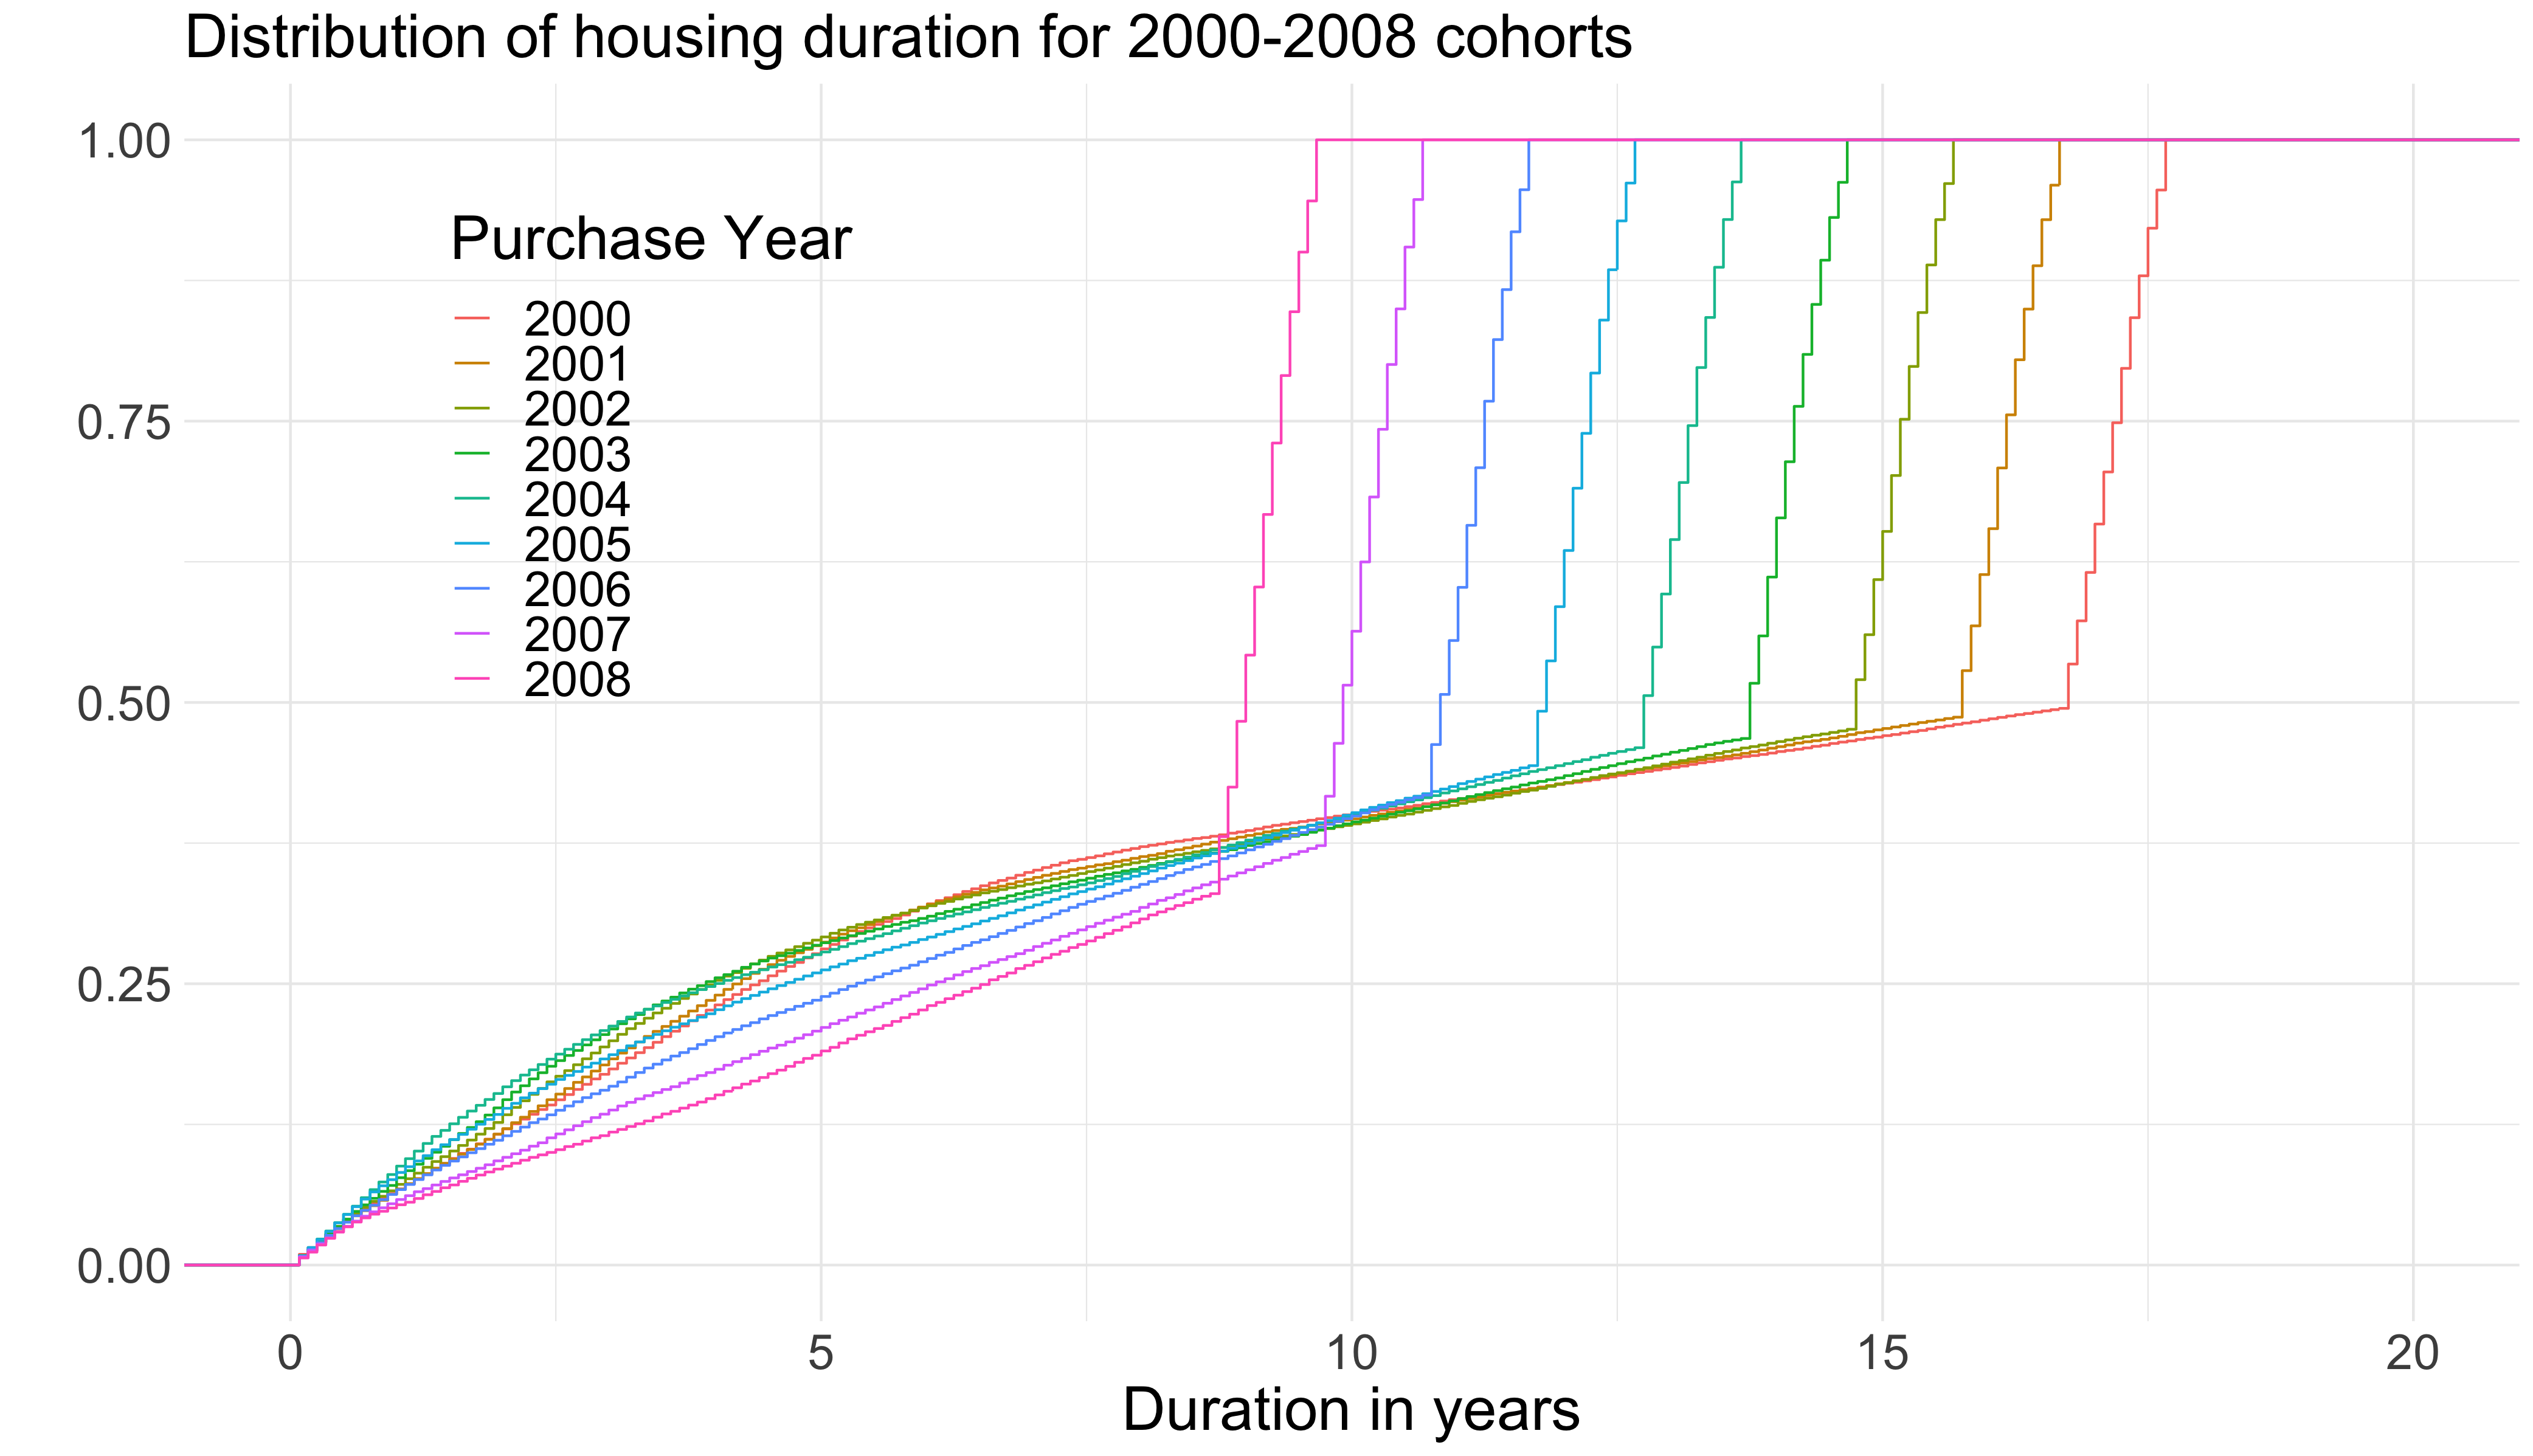
\includegraphics[width=\linewidth]{images/housing_duration_20002010_byyear_cdf.png}
  \end{column}
\end{columns}
\end{frame}


%%% PIVOT TO HAZARD MODELS
\begin{frame}{Pivoting to hazard models}
  \begin{wideitemize}
  \item We'll now discuss some parametric ways that papers address these problems
  \item   Duration modeling is, in many cases, focused on \emph{hazard} modeling. Why?
      \begin{itemize}
  \item Hazard has natural economic theory tie-ins
  \item Adjusts appropriately for the ``survival'' of individuals
  \end{itemize}
\item There is nothing more powerful in these settings than anything
  else we've studied -- by using parametric models, you are able to
  account for data issues, but require additional assumptions
  \end{wideitemize}
\end{frame}

\begin{frame}{Quick aside: some formal definitions}
  \begin{wideitemize}
  \item Let $F(y) = Pr(Y \leq y)$ be the probability of a duration no longer than $y$, and $f(y)$ the corresponding density
  \item Then, $S(y) = 1-F(y)$ is known as the survival function (the
    probability you'll survive until $y$)
  \item This lets us define the hazard function
    $h(y) = \frac{f(y)}{S(y)}$, which is the probability of an event
    occuring, condition on surviving until $y$.
  \item Key features of the hazard:
    \begin{itemize}
    \item Conditions on the population surviving until $y$ (rather
      than everyone)
    \item Can be time varying
    \item Summarizes all characteristics of $F$
    \end{itemize}
  \item Effectively think of it as a transformation of the distribution 
  \end{wideitemize}
\end{frame}


\begin{frame}{Why the hazard function? (Van Den Berg (2001))}
    \begin{columns}[T] % align columns
    \begin{column}{.4\textwidth}
      \begin{wideitemize}
      \item<1-> So why use a hazard model? E.g. extra structure
      \item<1-> Van Den Berg lays out some reasons in his Handbook chapter
        on duration modeling
        \begin{itemize}
        \item<1-> The hazard is a concise way to summarize the state
          of the remaining sample
        \item<2-> More effectively captures time-varying characteristics
        \item<2-> Deals well with right-censoring
        \end{itemize}
        \end{wideitemize}
    \end{column}%
  \hfill%
  \begin{column}{.6\textwidth}
    \begin{center}
      \only<1>{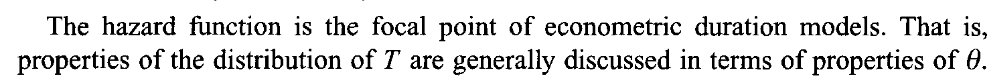
\includegraphics[width=\linewidth]{images/why_hazard1.png}\\
        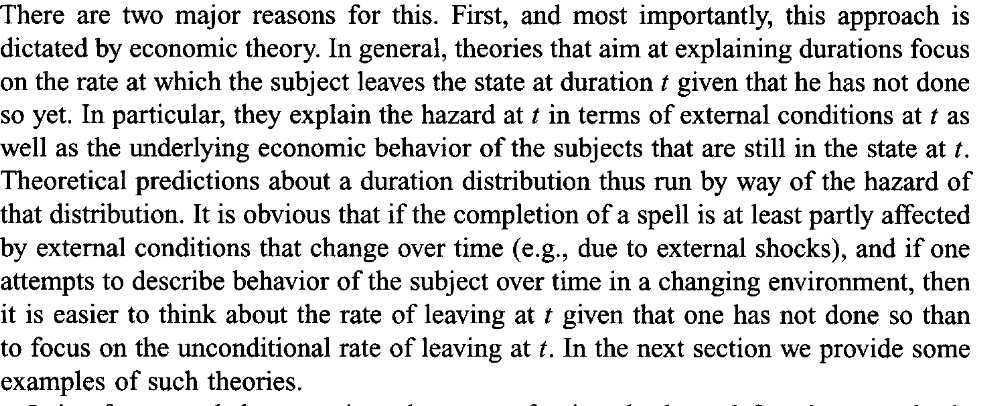
\includegraphics[width=\linewidth]{images/why_hazard2.png}}
      \only<2>{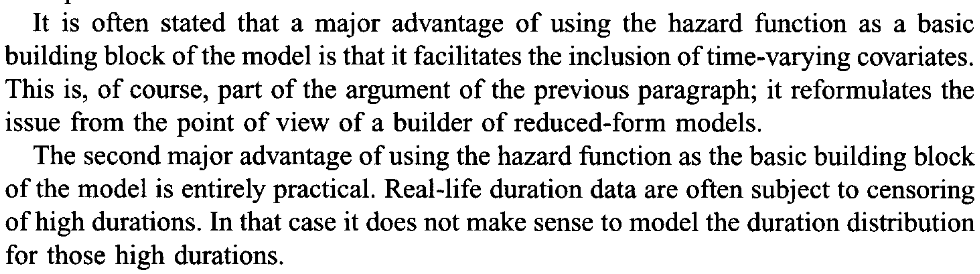
\includegraphics[width=\linewidth]{images/why_hazard3.png}}
    \end{center}
  \end{column}
\end{columns}
\end{frame}


\begin{frame}{Simple hazard example}
  \begin{wideitemize}
  \item Imagine that people move houses because of life events, and
    they arrive randomly with a random rate $\theta(t)$,
    \begin{itemize}
    \item the expected number of life events in a short time period is $\theta(t) dt$
    \item For now, assume it's constant -- e.g. $\theta = \theta(t)$
    \end{itemize}
  \item This implies a distribution of life events that is
    expontential with mean $1/\theta$:
    $$f(y) = \theta \exp(-y\theta) \text{ for } y > 0, \; F(y) = 1- e^{-\theta y}$$
  \item This distribution is extremely nice, since it has the lack of
    memory property, e.g.
    $$E(Y - c | Y > 0) = 1/\theta,$$
    irrespective of $c$
  \item Hence, the hazard rate is exactly $\theta$!
    
  \end{wideitemize}
\end{frame}

\begin{frame}{Hazard modeling data sampling}
  \begin{wideitemize}
  \item   We can use this setup to study our duration cases previously
  \item Consider our data sampling and the likelihood:
    \begin{itemize}
    \item With fully observed flow sampling, the likelihood is
      \begin{align*}
        L(\theta) &= \prod_{i=1}^{n} f(y_{i}|\theta) = \prod_{i=1}^{n} h(y_{i}|\theta) S(y_{i}|\theta)\\
        &= \prod_{i=1}^{n} \theta e^{-\theta y} \; \text{under exponential}
      \end{align*}
    \item With right censoring (not censored $\rightarrow$ $d_{i} = 1$) and flow sampling, the likelihood is
      \begin{align*}
        L(\theta) &= \prod_{i=1}^{n} f(y_{i}|\theta)^{d_{i}}S(c_{i}|\theta)^{1-d_{i}} = \prod_{i=1}^{n} h(y_{i}|\theta)^{d_{i}} S(y_{i}|\theta)^{d_{i}} S(c_{i}|\theta)^{1-d_{i}}\\
        \end{align*}
    \end{itemize}
  \end{wideitemize}
\end{frame}

\begin{frame}{Hazard modeling data sampling}
  \begin{wideitemize}
    \item With stock sampling, where you sample from the \emph{stock} of individuals (rather than the flow)
      \begin{itemize}
      \item A given draw is sampled to have lived for $s_{i}$ periods
      \end{itemize}
    \item Then,  the likelihood is
      \begin{align*}
        L(\theta) &= \prod_{i=1}^{n} \frac{f(y_{i}|\theta)}{S(s_{i}|\theta)} = \prod_{i=1}^{n} h(y_{i}|\theta) \frac{S(y_{i}|\theta)}{S(s_{i}|\theta)}\\
      \end{align*}
    \item With right censoring (not censored $\rightarrow$ $d_{i} = 1$) such that we do not track the observations, the likelihood is
      \begin{align*}
        L(\theta) &= \prod_{i=1}^{n} \left(\frac{f(y_{i}|\theta)}{S(s_{i}|\theta)}\right)^{d_{i}}\left(S(s_{i}|\theta)\right)^{(1-d_{i})}
      \end{align*}
  \end{wideitemize}
\end{frame}



\begin{frame}{Non-parametric estimations of survival with censoring}
  \begin{columns}[T] % align columns
    \begin{column}{.5\textwidth}
  \begin{wideitemize}
  \item<1-> In the full sample of the housing example, we were plotting the density of the
    variable $t_{i} = \min\{y_{i}, c_{i}\}$ 
  \begin{itemize}
  \item e.g., the true failure time or when it is censored
  \end{itemize}
\item<2-> However there's a lot of censoring in this full sample. How
  accurately does this map to the probability of someone staying in a
  home?
  \begin{itemize}
  \item E.g. can I use this to estimate $S(t) = Pr( Y_{i} > t)$?
  \end{itemize}
\item<2-> Short answer: not directly. Need to adjust for censoring and can do so
  non-parametrically
  \begin{itemize}
  \item We'll use the Kaplan-Meier estimator 
  \end{itemize}
  \end{wideitemize}
    \end{column}%
  \hfill%
  \begin{column}{.5\textwidth}
    \only<1>{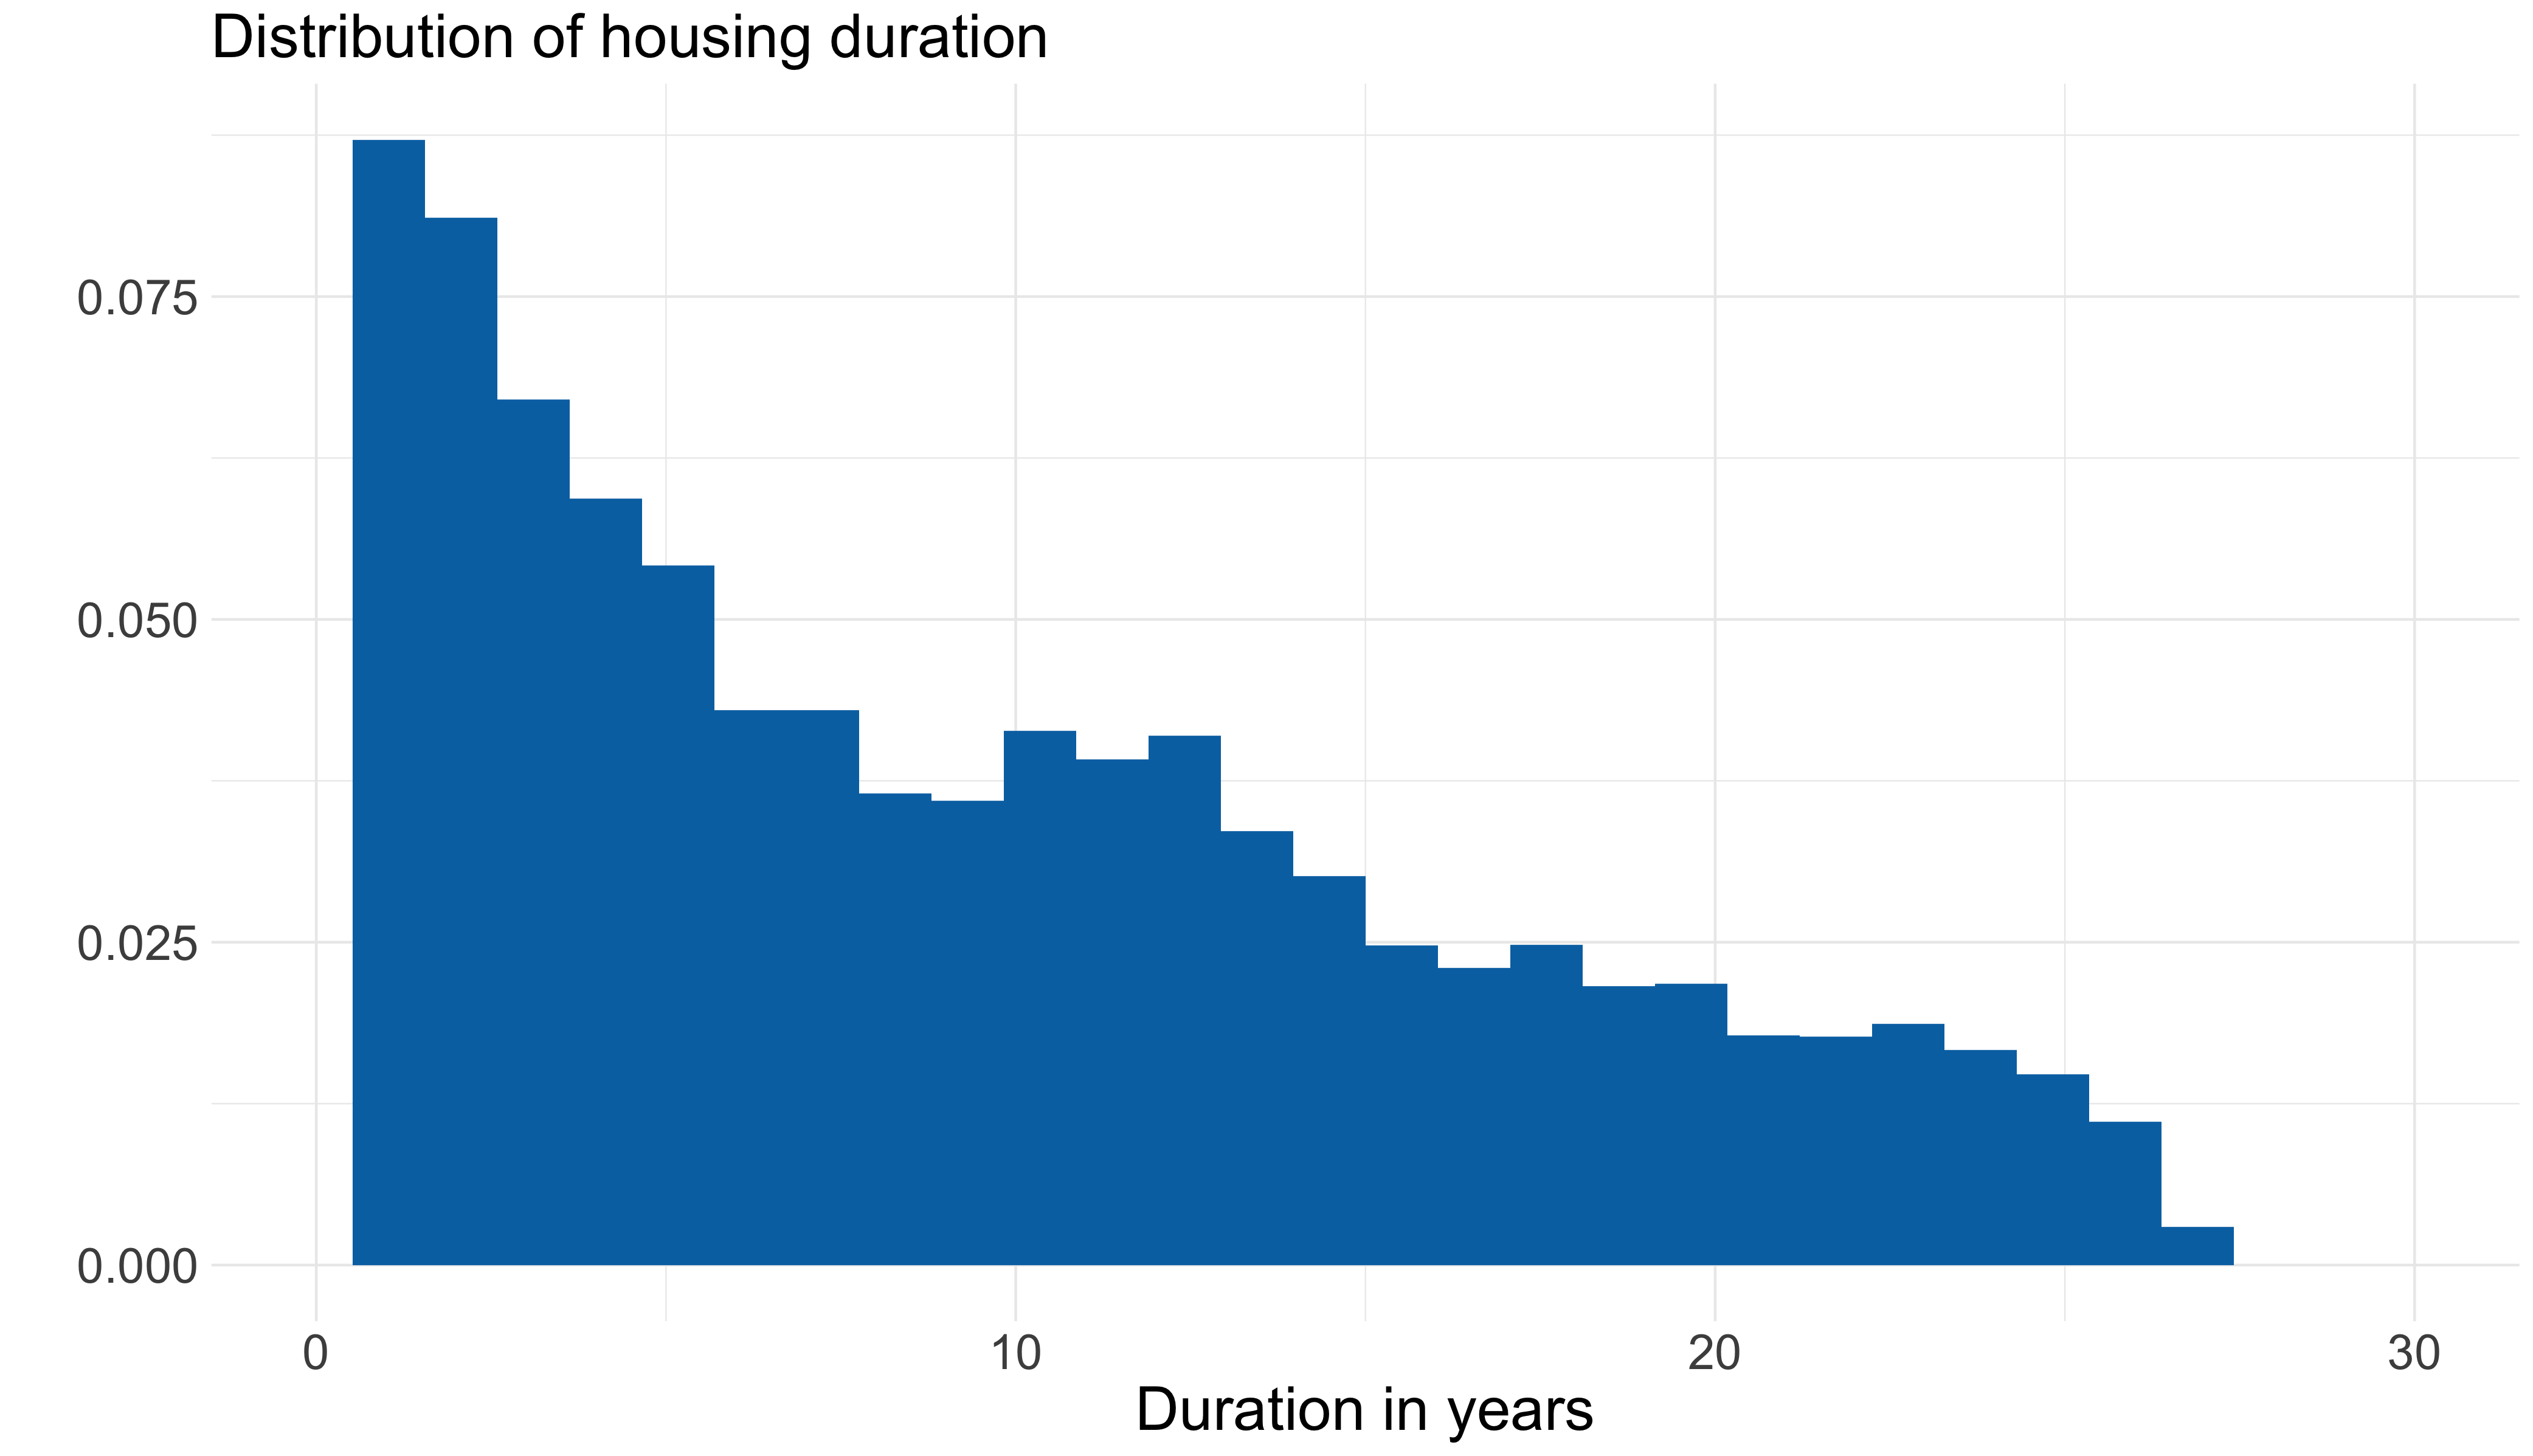
\includegraphics[width=\linewidth]{images/housing_duration_full.png}}
    \only<2>{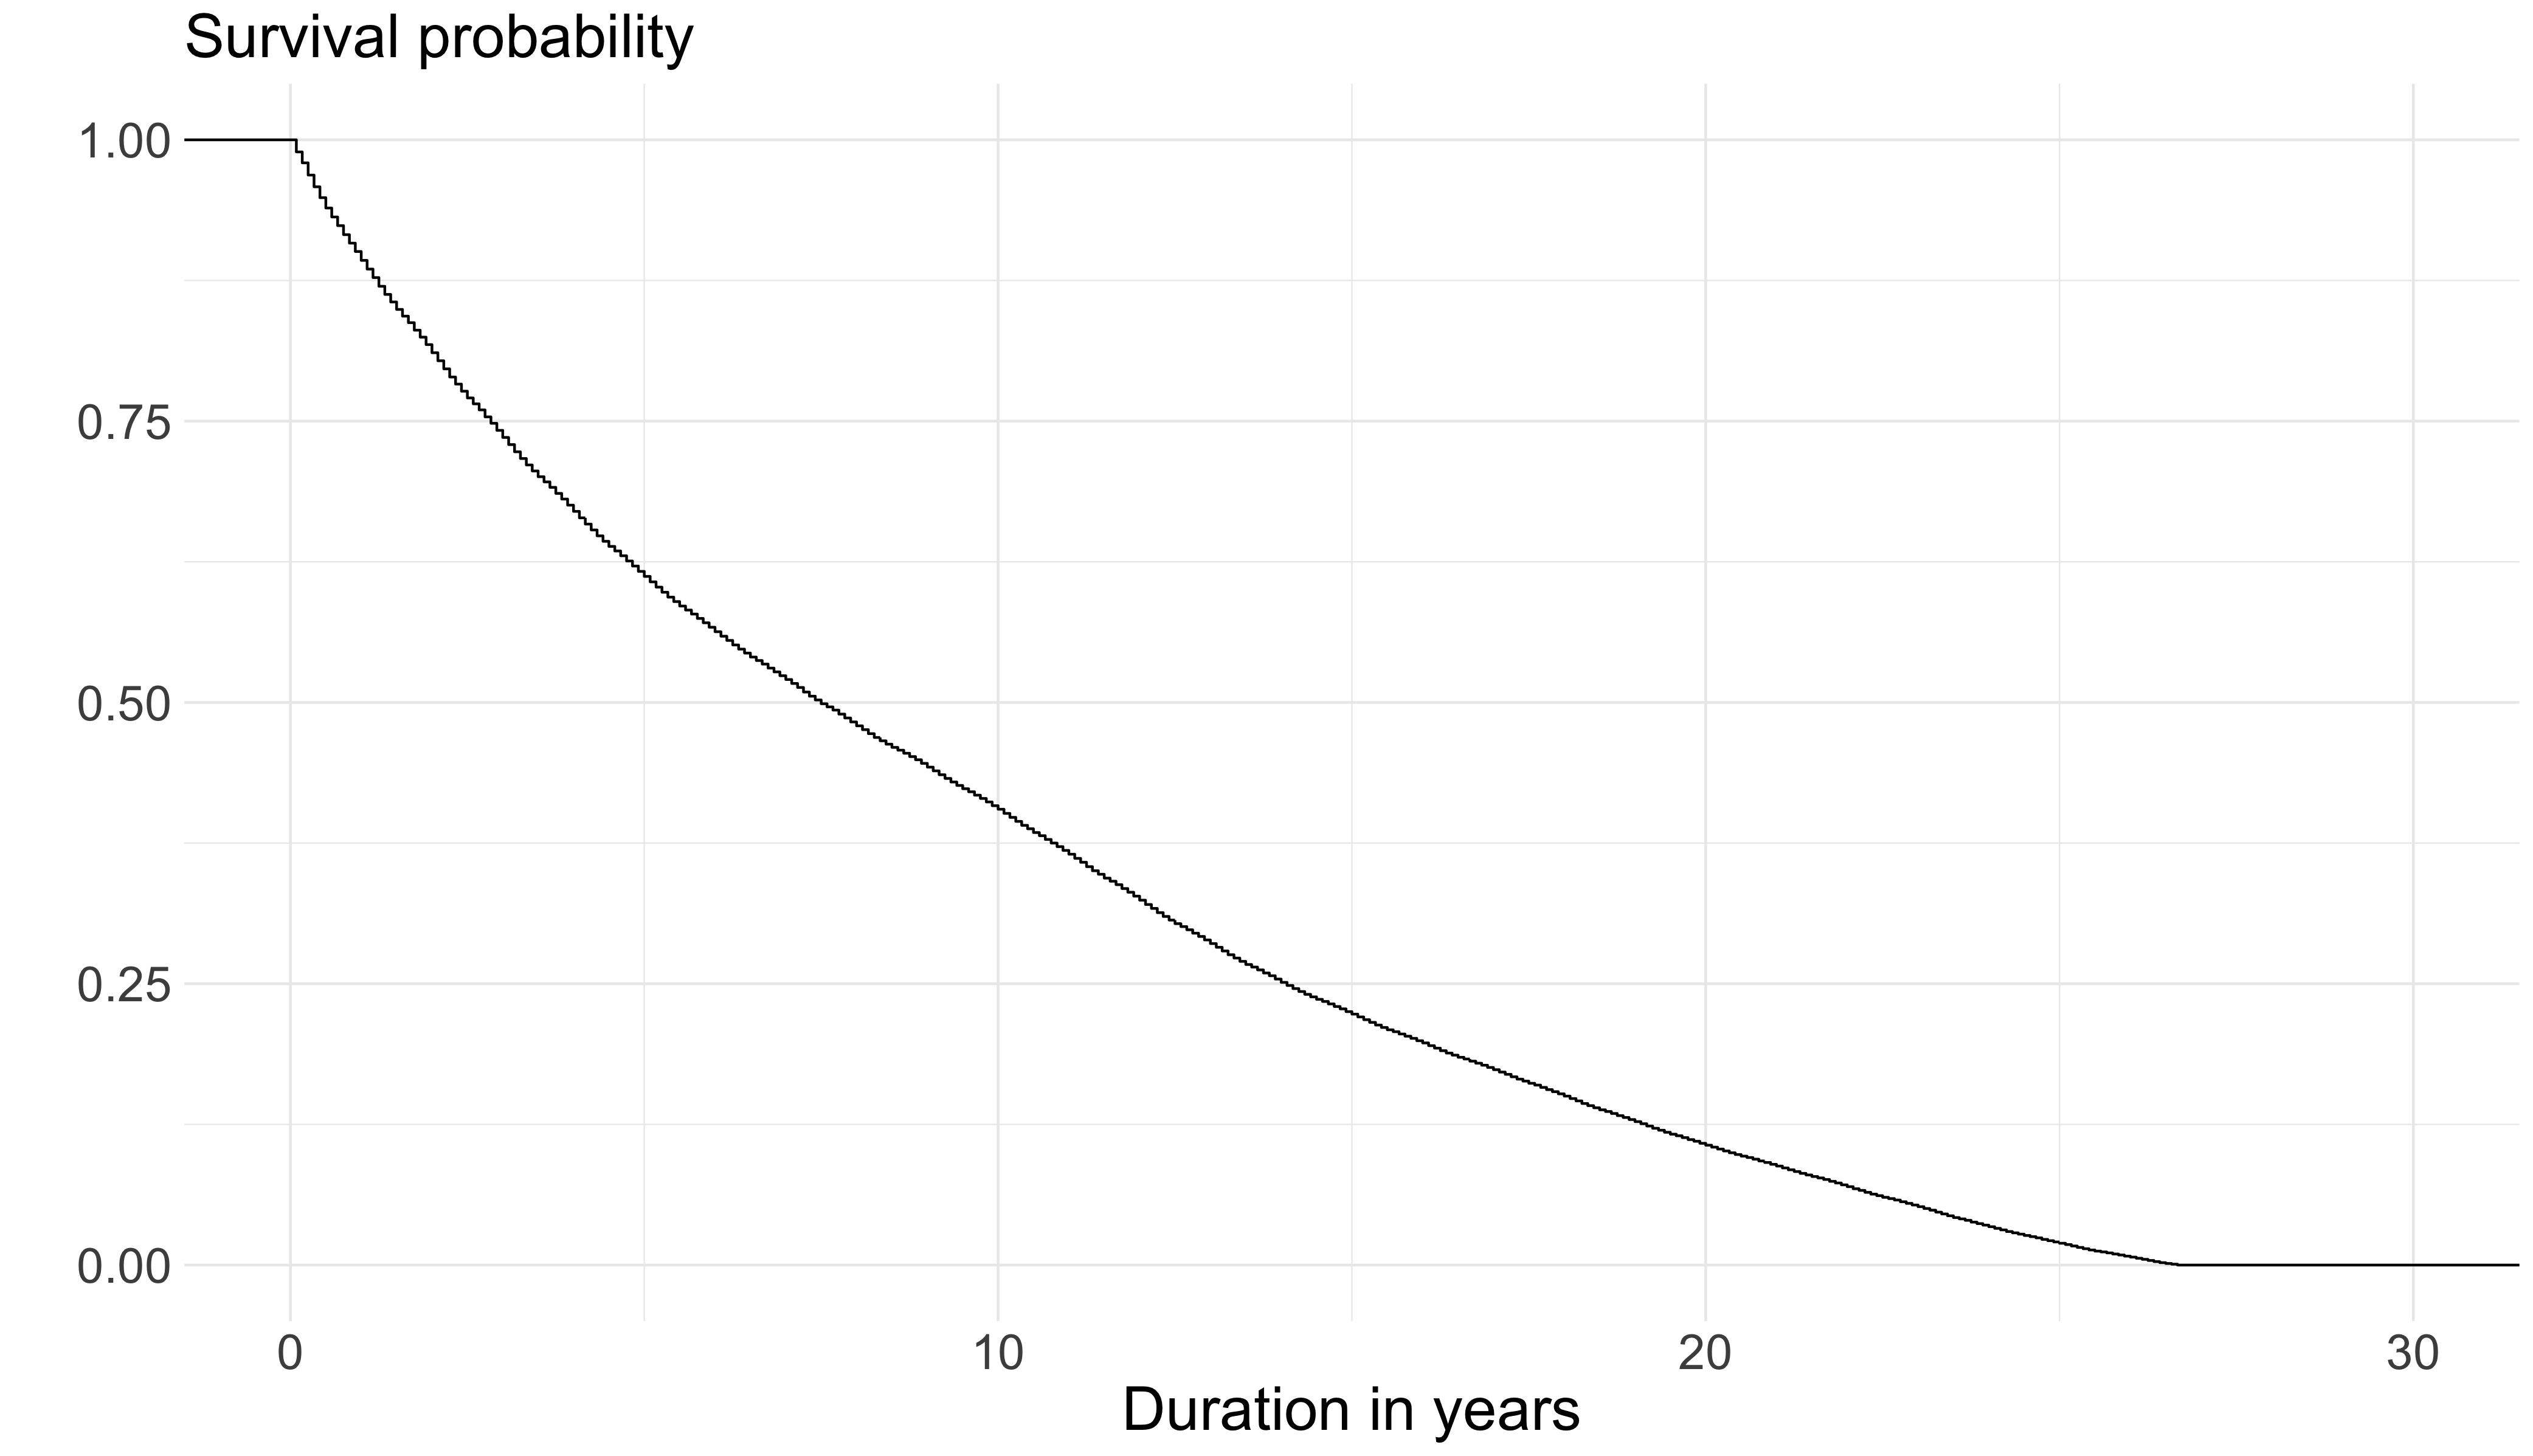
\includegraphics[width=\linewidth]{images/housing_duration_full_naive_survival.png}}
  \end{column}
\end{columns}
\end{frame}


\begin{frame}{Kaplan-Meier: non-parametric estimations of surival}
  \begin{columns}[T] % align columns
    \begin{column}{.8\textwidth}
      \begin{itemize}
      \item Kaplan-Meier estimator exploits the fact that the survival
        up to period $t$, $S(t)$, can be thought of as the joint
        probability of $t$ non-exits in a row:
        $S(t) = \prod_{j = 1}^{t}(1-h(j))$
      \item Then, this implies that
        $f(t) = h_{t}\prod_{j = 1}^{t-1}(1-h(j))$ and $f(1) = h(t)$.
      \item We need to just estimate $h(\cdot)$ for every time period.
        Let $a_{j} = \sum_{i} 1(Y_{i} \geq t) $,
        $e_{j} = \sum_{i} 1(Y_{i} = j \cap Y_{i} \leq c_{i})$
      \begin{align*}
        L(h) &= \prod_{i=1}^{n} f(y_{i})^{d_{i}}S(c_{i})^{1-d_{i}} \\
             &= \prod_{j} h_{j}^{e_{j}}(1-h_{j})^{a_{j}-e_{j}}
      \end{align*}
    \item Our MLE is $\hat{h}_{j} = e_{j}/a_{j}$
      \begin{itemize}
      \item Can consider standard errors and testing around these
        estimates
      \end{itemize}
  \end{itemize}
    \end{column}%
  \hfill%
  \begin{column}{.2\textwidth}
  \end{column}
\end{columns}
\end{frame}

\begin{frame}{Kaplan-Meier: non-parametric estimations of surival}
  \begin{columns}[T] % align columns
    \begin{column}{0.3\textwidth}
      \begin{itemize}
      \item Ignoring the censoring makes a big difference  
      \end{itemize}
    \end{column}%
  \hfill%
  \begin{column}{.7\textwidth}
    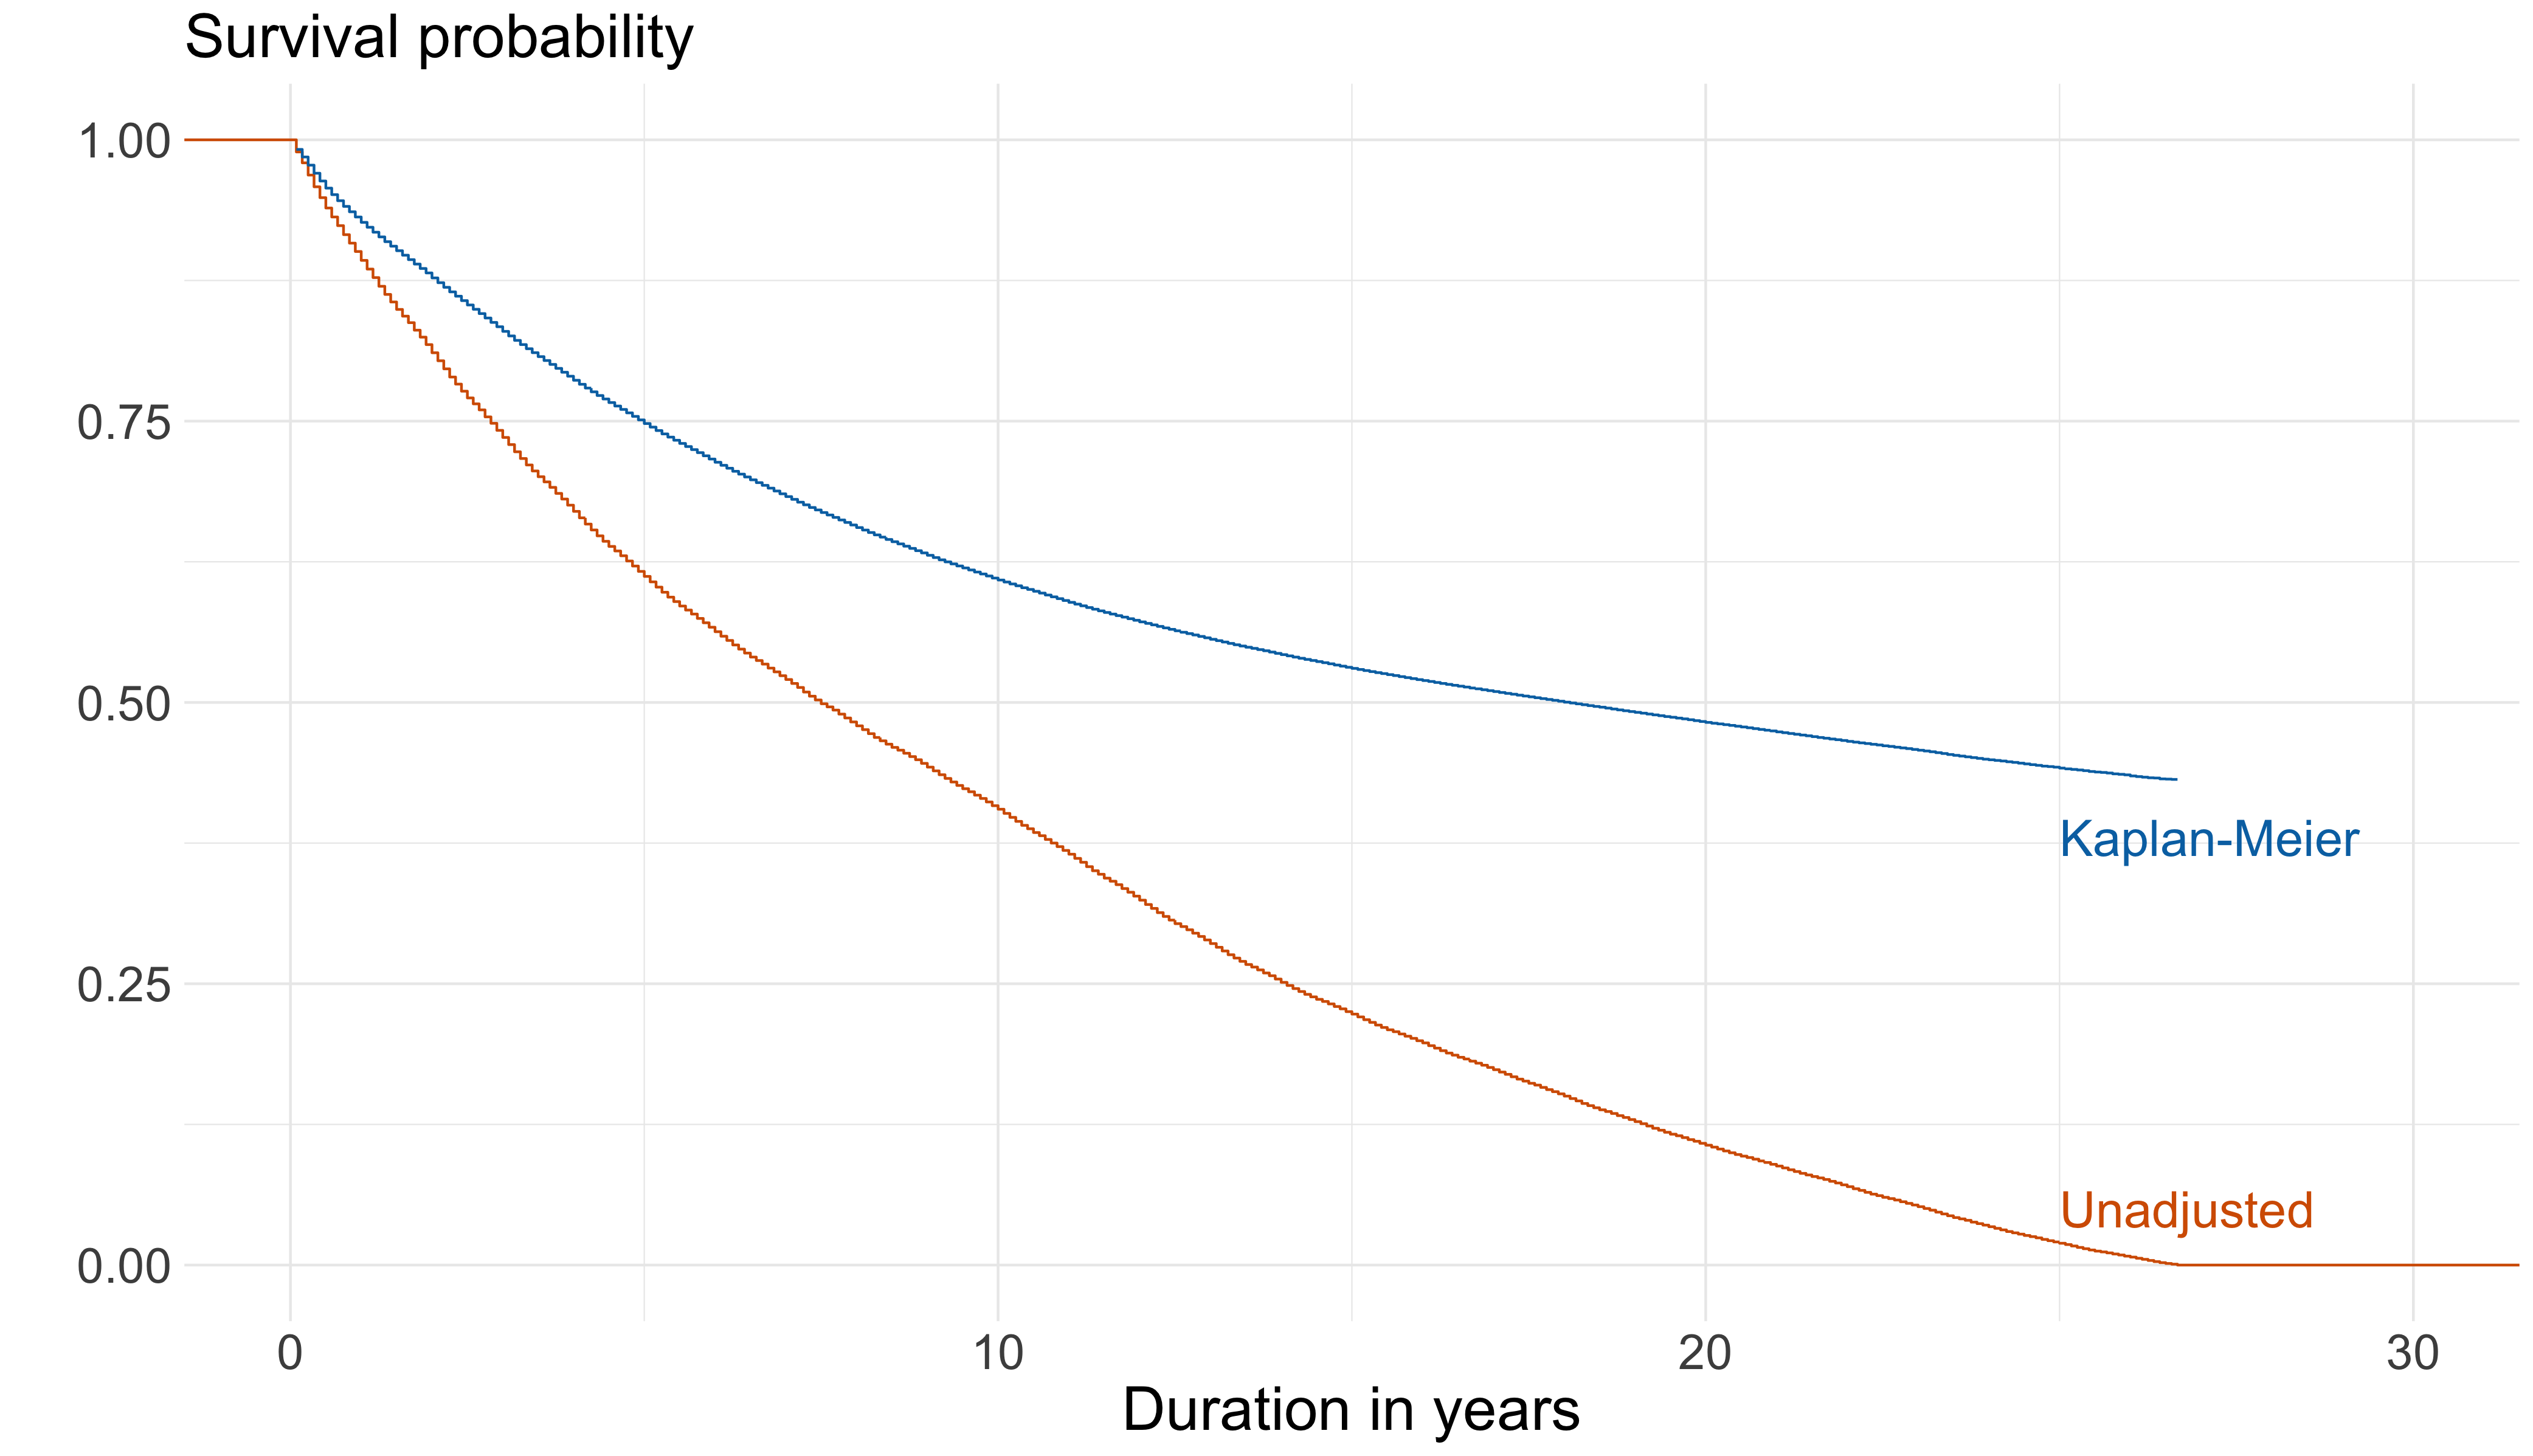
\includegraphics[width=\linewidth]{images/housing_duration_full_naive_survival_v_KM.png}
  \end{column}
\end{columns}
\end{frame}


\begin{frame}{Hazard modeling data sampling}
  \begin{wideitemize}
  \item Clearly, ignoring the censoring will bias your estimates -
    either of $\theta$ in a parameterized model, or of $h(t)$ in
    non-parametric estimates
    \begin{itemize}
    \item There are two ways one could naively ignore it -- toss any
      data that's censored, or treat the censoring as real data
    \item Both will give over-estimates of $\theta$ in the exponential case
    \end{itemize}
  \item To see the intuition, let $t_{i} = min(y_{i}, c_{i})$, and
    note the likelihood.
    \begin{align*}
      L(\theta) &= \prod_{i=1}^{n} h(t_{i}|\theta)^{d_{i}} S(t_{i}|\theta)
    \end{align*}
  \item Now assume the exponential and solve for the MLE
    $\hat{\theta} = \overline{d}/\overline{t}$. Consider how
    the estimates change if you either throw out data, or mislabel
    the censoring
    \begin{itemize}
    \item If you ignore the censoring, $\overline{d} \rightarrow 1$,
      and $\overline{t}$ doesn't change. Upward bias in
      $\hat{\theta}$
    \item If you drop the censored obs, then the MLE is
      $\bar{\theta} = \sum d_{i} / \sum d_{i} t_{i}$ Note that the
      numerator remains unchanged, but the denominator
      decreases. Upward bias in $\hat{\theta}$
    \end{itemize}
  \end{wideitemize}
\end{frame}


\begin{frame}{Value of hazard modeling}
  \begin{wideitemize}
  \item So far, the main value of the modeling is to add parametric
    structure to capture the univariate features of duration
    \begin{itemize}
    \item E.g., we want to know the properties of a censored random variable
    \end{itemize}
  \item However, in many cases we want to know the effect of some
    variable on the duration
    \begin{itemize}
    \item E.g. $Y = D\beta + \epsilon$
    \end{itemize}
  \item What is the downside of simply running a regression like
    above? As Van Den Berg discusses above:
    \begin{itemize}
    \item Hazard rate will more concisely capture a meaningful
      characteristic
    \item Time-varying characteristics are more easily accomodated
      (e.g., how does the above linear regression incorporate a
      changing minimum wage schedule?)
    \item The simple linear regression approach doesn't deal with
      censoring well
    \end{itemize}
  \end{wideitemize}
\end{frame}

\begin{frame}{A defense of regression}
  \begin{wideitemize}
  \item An aside in defense of a simple linear regression approach
  \item While hazard modeling is tightly connected to economic
    models, it can feel non-transparent (as many non-linear models
    do)
  \item Simple linear regression models \emph{can} address censoring in two ways:
    \begin{itemize}
    \item Indicators of ``survived to year $K$'' , so long as year
      $K$ is not censored
    \item quantile regression
    \end{itemize}
  \item It is possible to use these combinations to do a number of
    robust analyses
    \begin{itemize}
    \item In fact, I would highly recommend that any hazard modeling
      done is also supported by simple linear regression as well
    \end{itemize}
  \item However any linear regression needs to be \emph{extremely}
    aware of the data sampling process
  \end{wideitemize}
\end{frame}

\begin{frame}{The workhorse of hazard modeling - Proportional Hazard}
  \begin{wideitemize}
  \item In some settings, there is theory driving the hazard
    modeling, and that should determine your approach
    \begin{itemize}
    \item in more reduced form settings, you need a workhorse model that
      is flexible
    \end{itemize}
  \item In hazard models, this model is the Cox proportional hazards model:
    \begin{equation}
      \theta(t | x) = \phi(t) \theta_{0}(x) , 
    \end{equation}
    where $\theta_{0} = \exp(x\beta)$ usually. $\phi(t)$ is the
    \emph{baseline} hazard, and gives the underlying shape of the
    hazard function.
  \item The characteristics of individuals $x$, move around the
    level of the hazard curve, but do not change the overall shape
    (e.g. $\theta_{0}$ is not directly a function of time, other
    than through $x$)
  \item In more complicated settings, we can allow for unobserved
    heterogeneity $v$ in what is known as the \emph{mixed} proportional
    hazards model:
    \begin{equation}
      \theta(x|t, v) = \phi(t) \theta_{0}(x) v
    \end{equation}
    
  \end{wideitemize}
\end{frame}

\begin{frame}{Unobserved heterogeneity}
  \begin{equation}
    \theta(x|t, v) = \phi(t) \theta_{0}(x) v
  \end{equation}
  
  \begin{wideitemize}
  \item   Key result from Lancaster that is easy to understand - hazard rate could be time varying (which is interesting from a theoreteical point) or it could be unobserved heterogeneity
  \item Consider the following example. Suppose there are two
    types of people in the population, ``movers'' and ``stayers'',
    movers are share $p$ and stayers $1-p$. Movers have a of
    $\theta_{m}$ = 2. Stayers have a lower lower rate of
    $\lambda_{s} = 1$.
  \item As time goes on, the share of each in the remaining
    population changes, shifting the overall hazard rate
    \begin{itemize}
    \item However, it's not that hazard rates are changing, but
      instead a compositional impact of unobserved heterogeneity
    \end{itemize}
  \item Using multi-spell data is a way to address this issue,
    similar to panel data with unobserved heterogeneity
    \begin{itemize}
    \item See Van Den Berg (2001) and Rose (2020) for details on cites
    \end{itemize}
  \end{wideitemize}
\end{frame}

\begin{frame}{Estimation}
  \begin{wideitemize}
  \item This approach, as with the simple hazard model, uses likelihood methods
  \item The key complications are:
    \begin{itemize}
    \item The baseline hazard model
    \item The heterogeneity
    \end{itemize}
  \item How to deal with the baseline hazard? $\lambda(t)$ is a
    nuisance parameter for the estimation of the $\theta_{0}$.
  \item The Cox approach ($v = 1$) for the nuisance parameter
    exploits the proportionality: at any given event, the
    \emph{partial likelihood} for unit $i$ that fails at period
    $t$ is
    \begin{align*}
      L_{i}(\beta) &= \frac{\phi(t)\theta_0(X_{i}\beta)}{\sum_{j : Y_{j} > Y_{i}} \phi(t)\theta_0(X_{j}\beta)}\\
                   &= \frac{\theta_0(X_{i}\beta)}{\sum_{j: Y_{j} > Y_{i}} \theta_0(X_{j}\beta)}
    \end{align*}
    (this is analogous to the solution in conditional logit)
  \end{wideitemize}
\end{frame}

\begin{frame}{Simplifying the intuition}
  \begin{columns}[T] % align columns
    \begin{column}{0.3\textwidth}
\only<1>{  \begin{wideitemize}
    \item In the case on a non-time-varying treatment (e.g. a baseline
      covariate) that is binary (or discrete), we don't need to get quite so complicated
    \item What if we just compared Kaplan-Meier survival functions?
      \begin{itemize}
      \item Let's compare boom and bust houses
      \end{itemize}
    \end{wideitemize}}
  \only<2>{
    \begin{itemize}
    \item Very intuitive and straightforward to compare hazards
    \item Doesn't look like proportional hazards is a reasonable
      assumption
      \begin{itemize}
      \item This is a standard model fit check
      \end{itemize}
    \item Key downside: doesn't accomodate unobserved heterogeneity,
      nor time-varying characteristics
    \end{itemize}}
    \end{column}%
  \hfill%
  \begin{column}{.7\textwidth}
    \only<1>{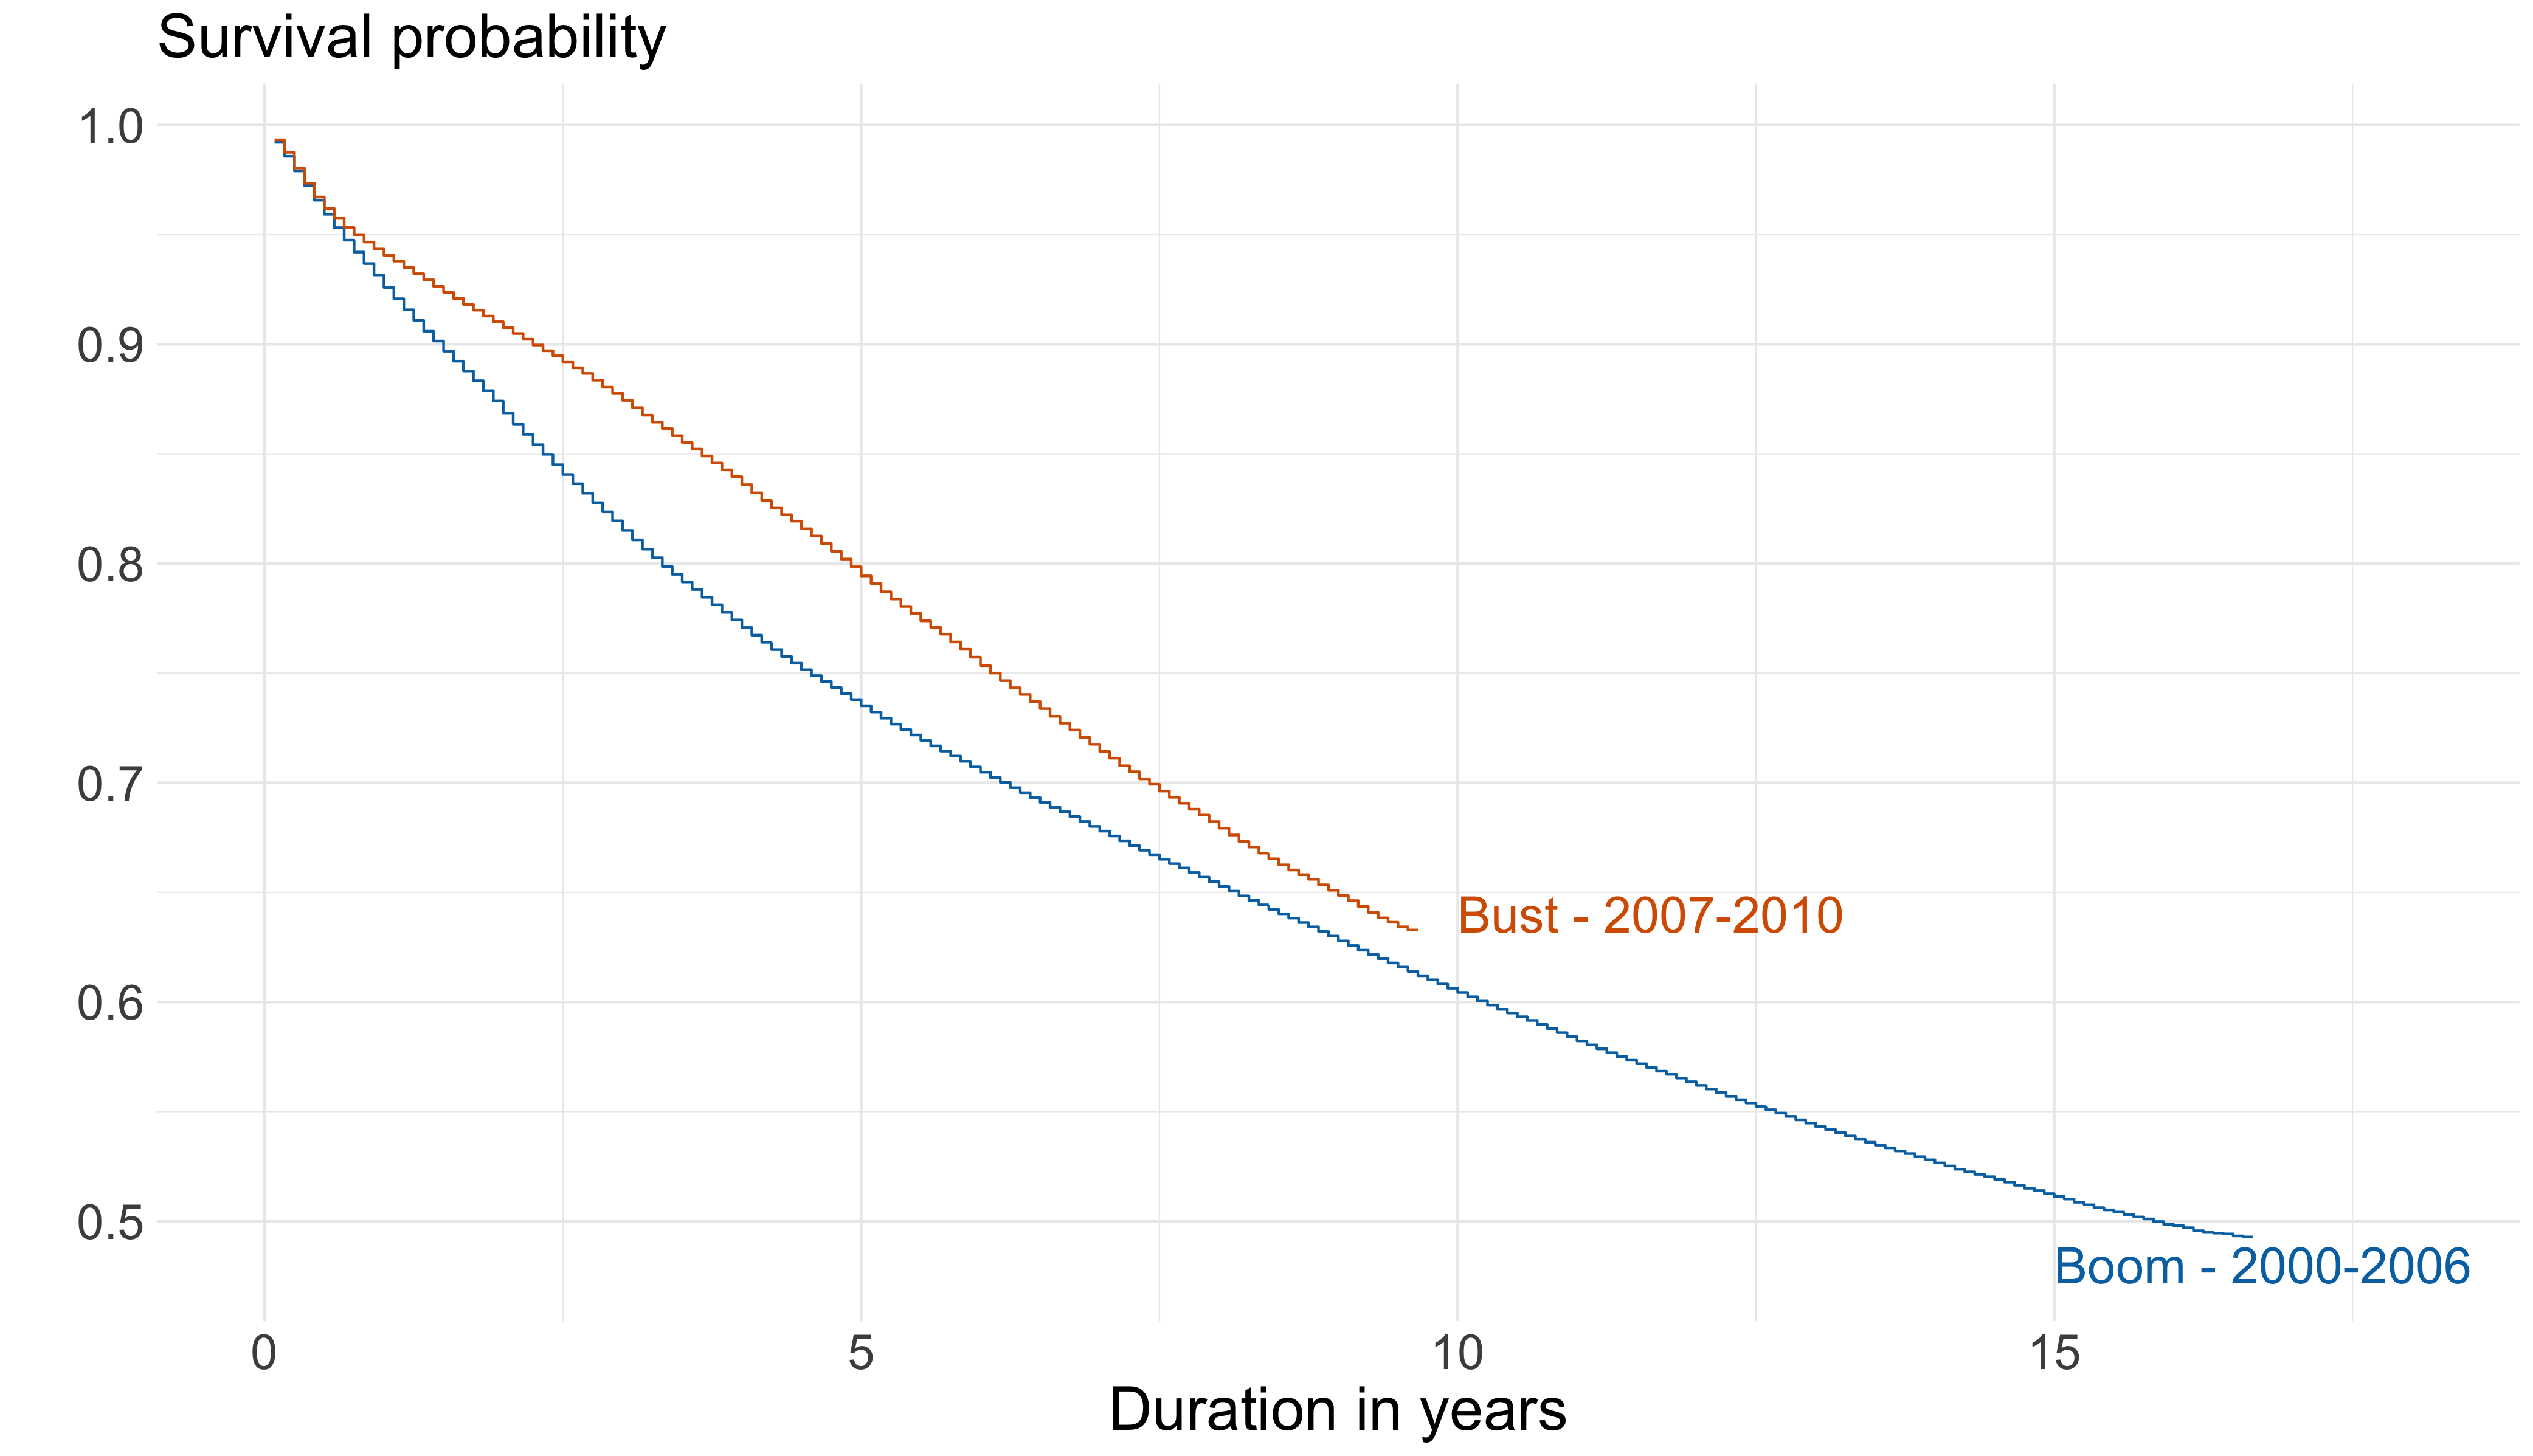
\includegraphics[width=\linewidth]{images/housing_duration_survival_KM_boom_bust.png}}
    \only<2>{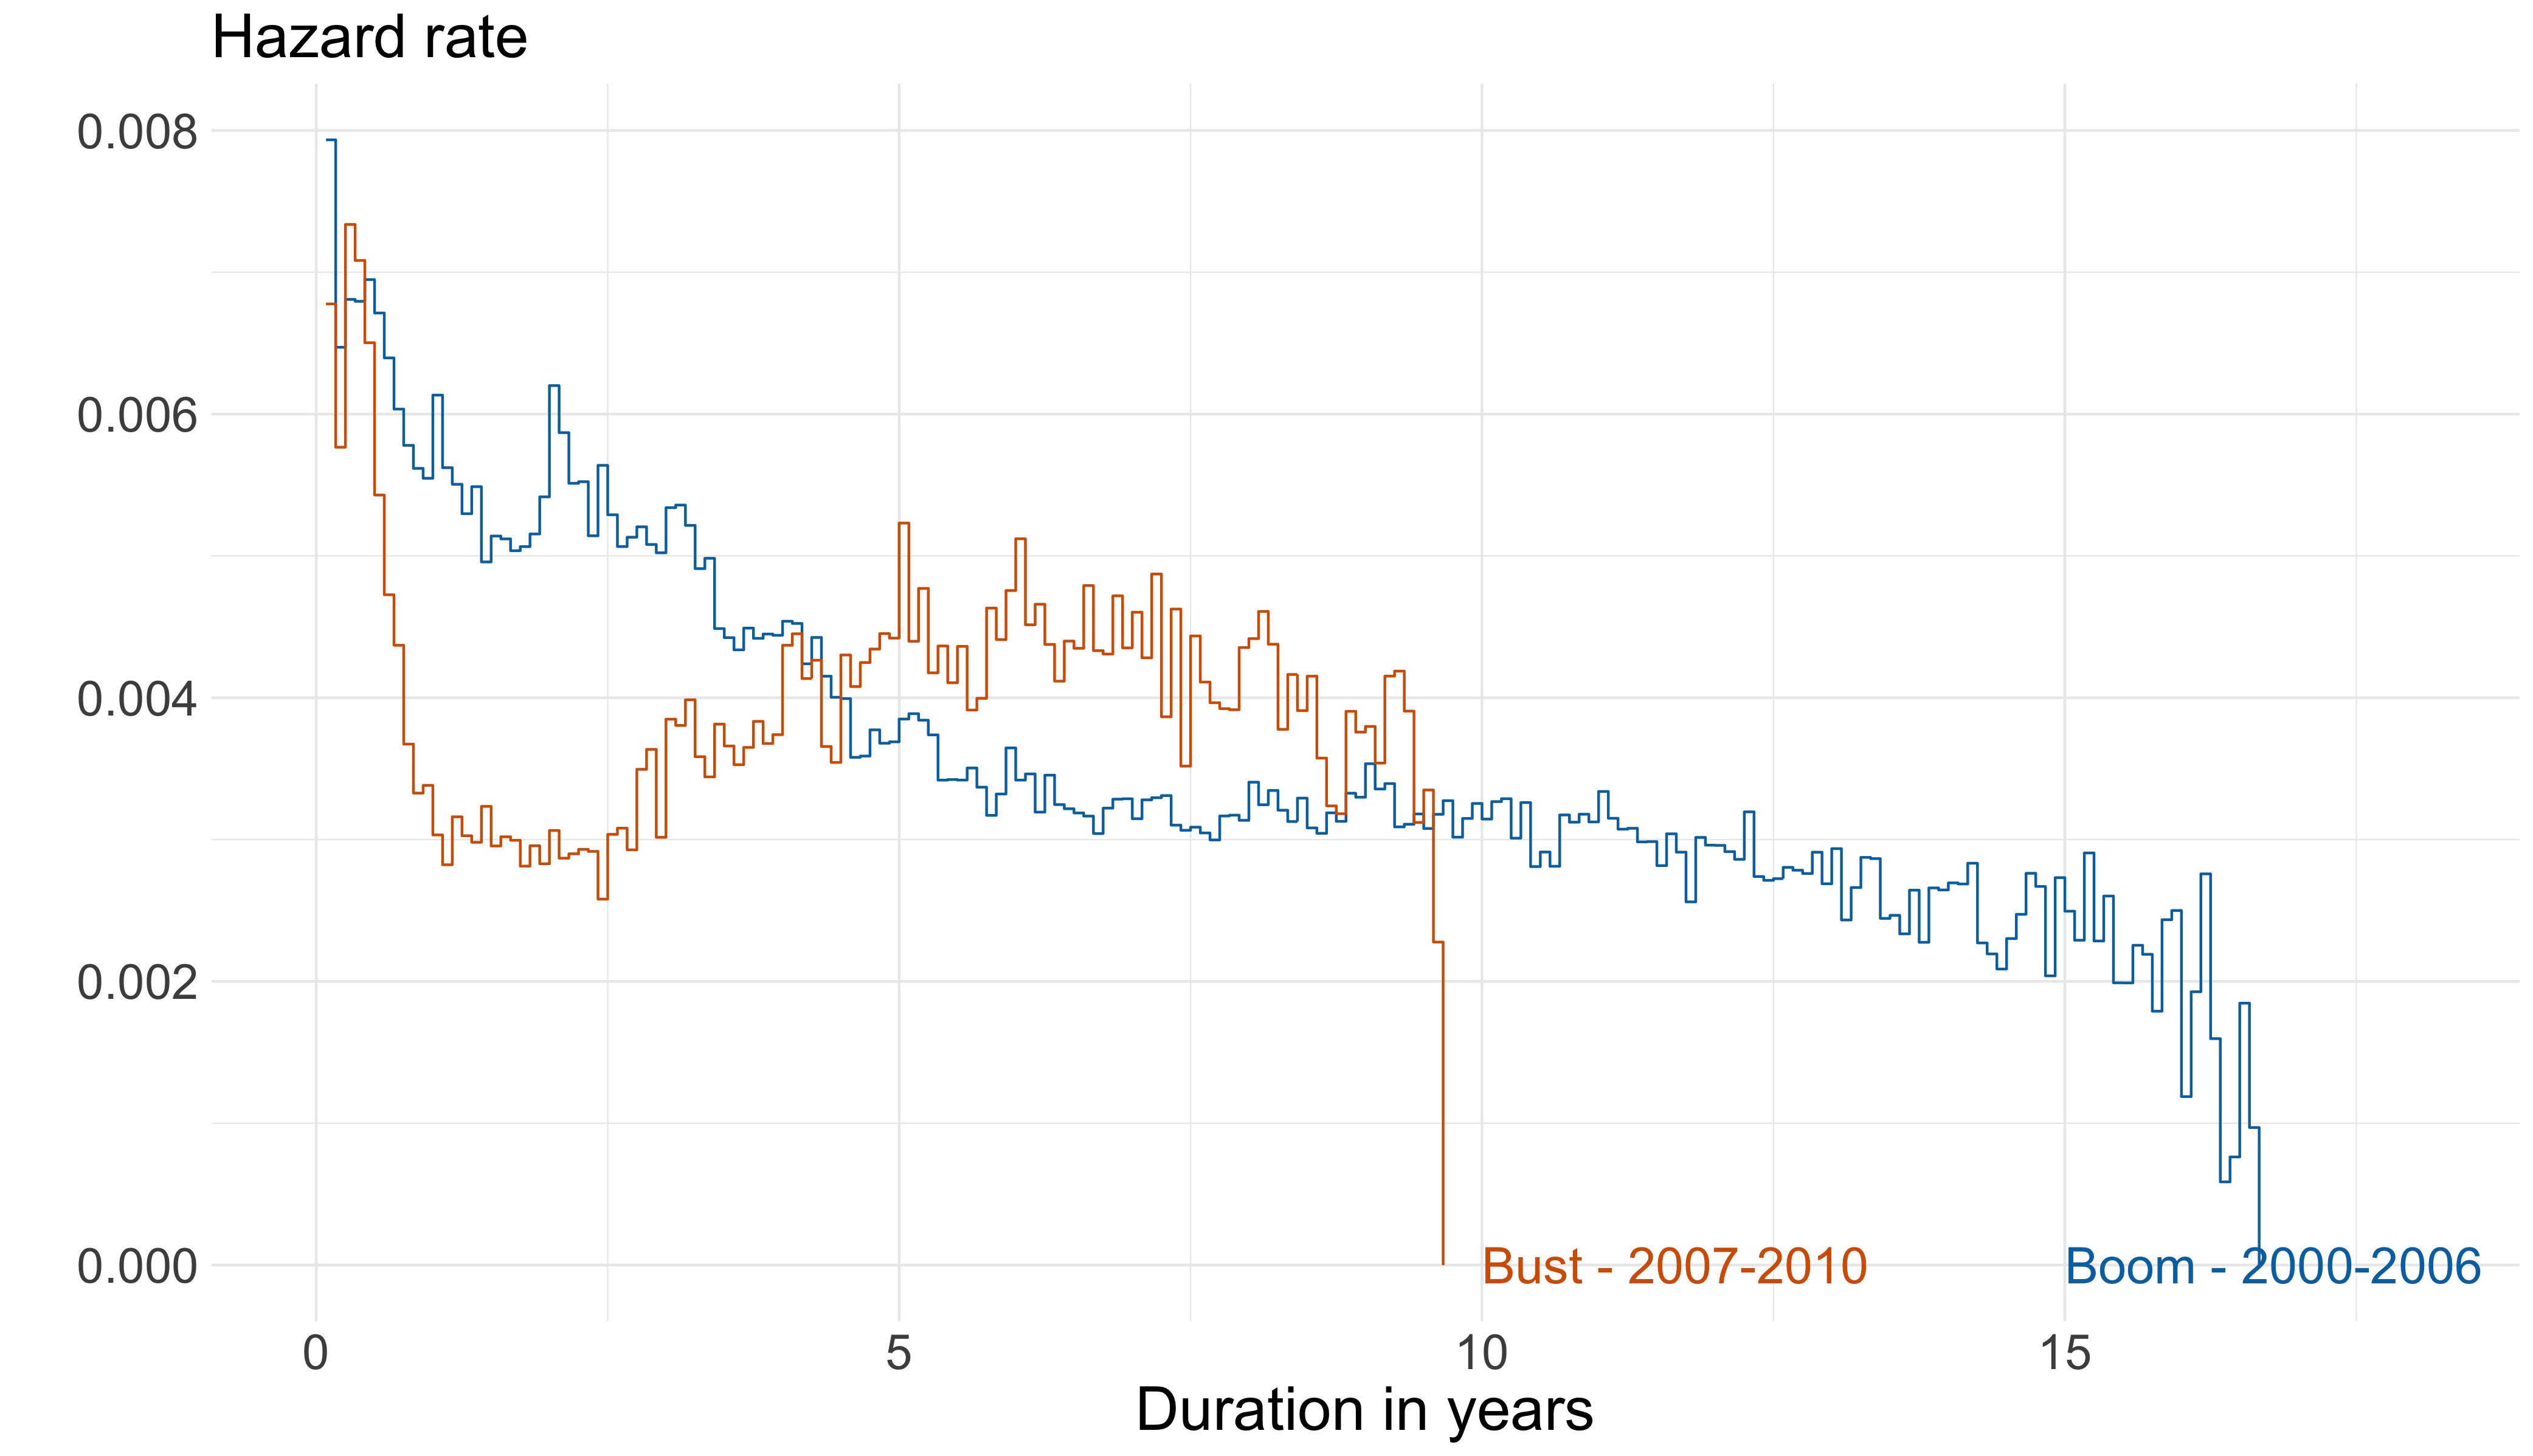
\includegraphics[width=\linewidth]{images/housing_duration_hazard_KM_boom_bust.png}}    
  \end{column}
\end{columns}
\end{frame}

\begin{frame}{Sometimes you have to get complicated}
  \begin{columns}[T] % align columns
    \begin{column}{0.9\textwidth}
      \begin{wideitemize}
      \item Sometimes a more complicated model is worthwhile, and you can't do a simple comparison
        \begin{itemize}
        \item Time-varying treatments being an obvious case
        \end{itemize}
      \item Key tension (discussed in Abbring and Van Den Berg (2003))
        -- when is the \emph{timing} of the time-varying treatments?
        \begin{itemize}
        \item Anticipation of treatments will confound your estimates
        \end{itemize}
      \item Additional complicating factor: competing risks
        \begin{itemize}
        \item What if there are multiple simultaneous states one could transition to?
        \item e.g. Unemployment could go to employment, or leaving the labor force
        \item e.g. Mortgage could go to default or prepayment
        \item Our strategies above ignore this and assume the risks
          are independent
          \begin{itemize}
          \item This is clearly a strong assumption
          \end{itemize}
        \end{itemize}
      \item See Honore and Lleras-Muney (2006) for a discussion on the
        fundamental identification issue in competing risks
      \end{wideitemize}
    \end{column}%
    \hfill%
    \begin{column}{.7\textwidth}
    \end{column}
  \end{columns}
\end{frame}


\end{document}